% !TEX root = thesis.tex
\section{Systematic erros}
{\color{red} Extend Systematics}
\label{sec:systematicerrors}
The systematic uncertainties in this analysis come from the background estimation, the unfolding procedure and the cuts used to select the tracks. Tracking uncertainties are estimated from variations of the track selection cuts defined in Sec.~\ref{sec:experimentaldetails}. The resulting variations in RMS are shown in Table \ref{tab:systematics}. The uncertainties from unfolding and background subtraction are of the same magnitude. 

The systematics in background estimation were studied using an alternative method to extract the background, mainly the random background method. The resulting uncertainty is below 5\% for the wide component RMS and below 9\% for the narrow component RMS. 

The systematic uncertainty that arises from the unfolding procedure is estimated by performing the unfolding with two separate methods. Data corrected by the iterative unfolding method are used as the results and the SVD unfolding method is employed to estimate the uncertainty. In a \textsc{Pythia} closure test the true distribution was in general found to be between the unfolded distributions from the iterative and SVD method. The difference between the methods when unfolding data should give a reasonable estimate of the unfolding uncertainty. The resulting uncertainty is below 8\% for both wide and narrow component RMS.

The different source of the systematic uncertainty are considered as uncorrelated and the values of each source are summed in quadrature. The resulting uncertainty is 9 \% for the wide component RMS and 12 \% for the narrow component RMS. 

\begin{table}[htb]
\centering
\caption{Summary of systematic errors}
\label{tab:systematics}
\begin{tabular}{ l | c | r }
  Systematic & Wide RMS & Narrow RMS \\
    \hline			
  Background & 5 \% & 9 \% \\
  Unfolding & 8 \% & 8 \% \\
  Tracking & ? \% & ? \% \\
  Total & 9 \% & 12\% \\
  \hline
  \end{tabular}
  \end{table}
  
  \subsection{Background}
 Fits are performed on both perpendicular cone and random background signals. Difference between them is taken as the systematic error. The fits for individual bins from the random background method are shown in figure \ref{fig:fitsrandombg}. Resulting differences between the methods for different components are shown in figure \ref{fig:systbg}.




\begin{figure}
\centering
\begin{subfigure}{0.24\textwidth}
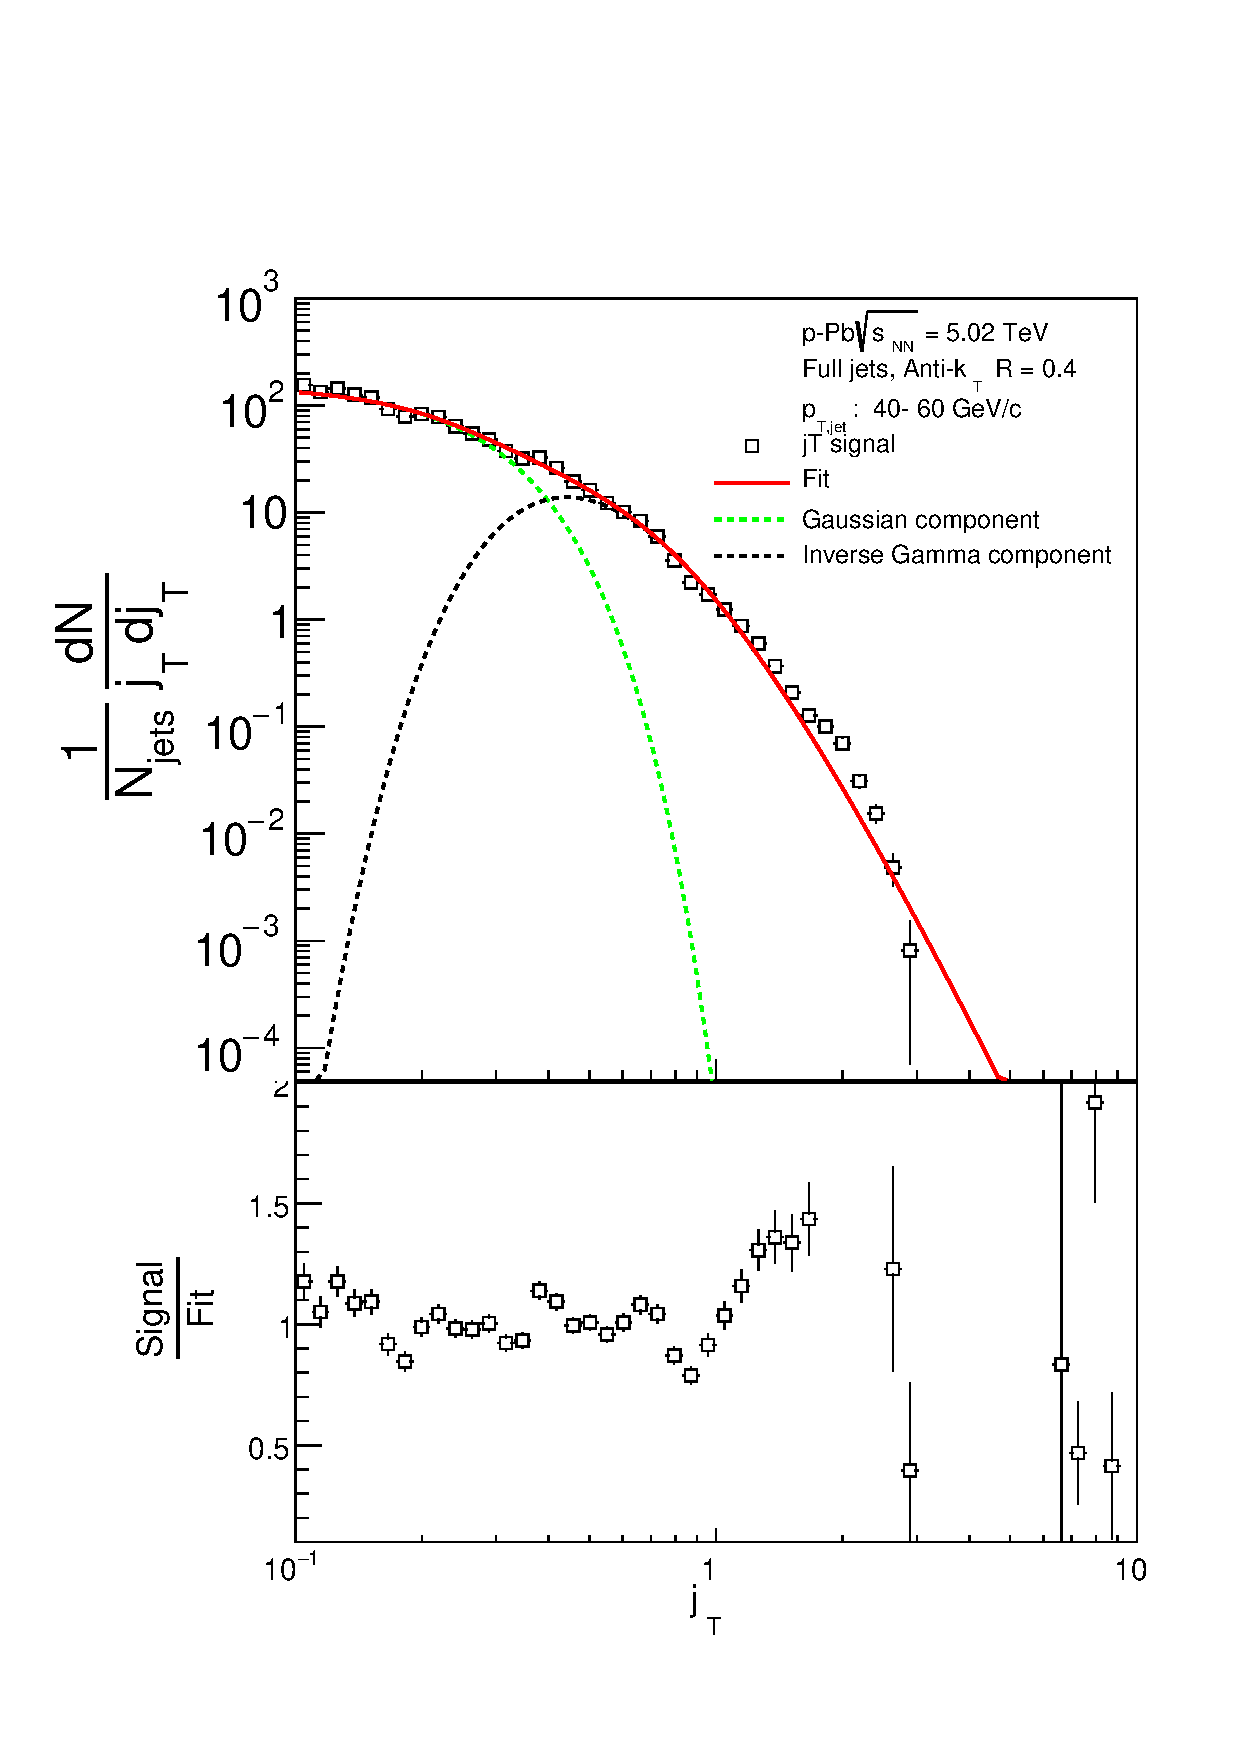
\includegraphics[width=0.95\textwidth]{results/JetConejTSignalFit/JetConejTSignalFitNFin00JetPt04randomBgBayes}
\end{subfigure}
\begin{subfigure}{0.24\textwidth}
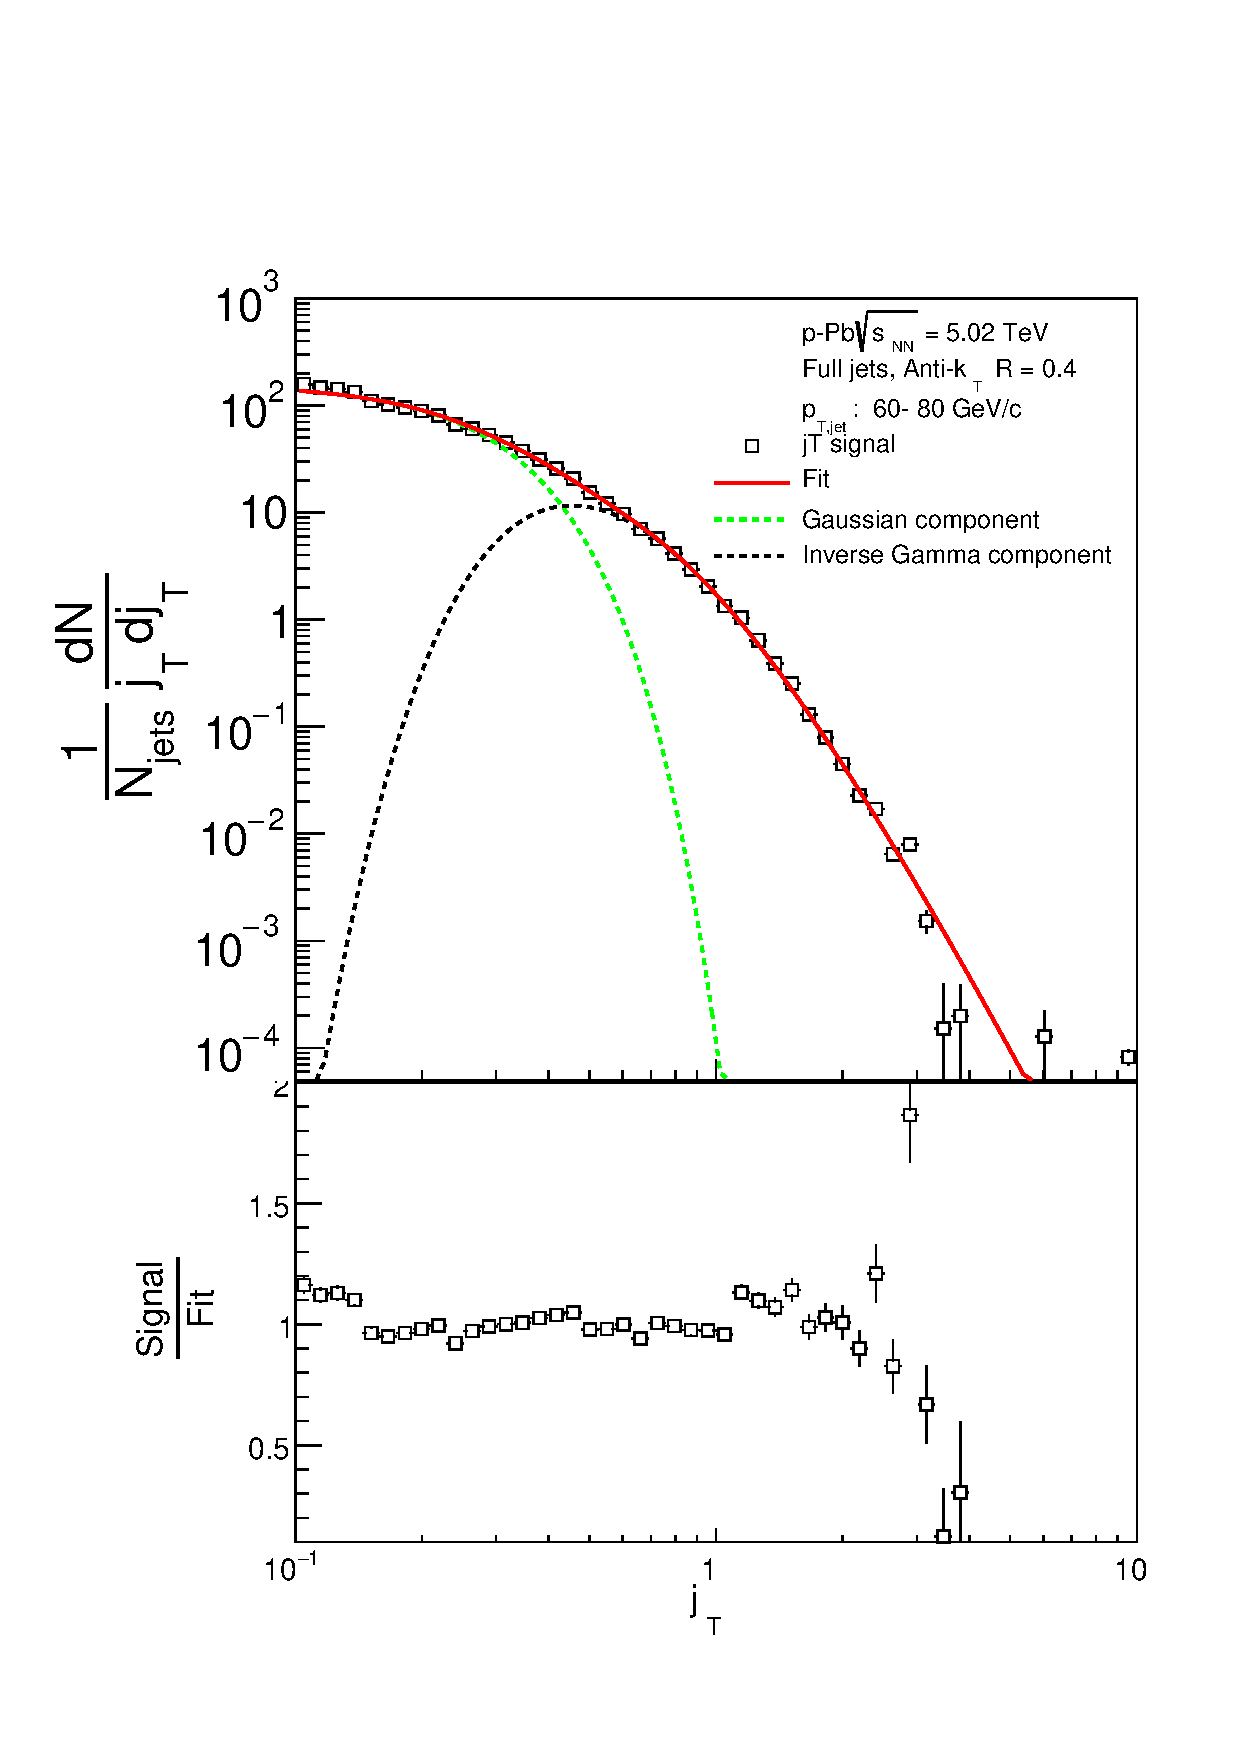
\includegraphics[width=0.95\textwidth]{results/JetConejTSignalFit/JetConejTSignalFitNFin00JetPt05randomBgBayes}
\end{subfigure}
\begin{subfigure}{0.24\textwidth}
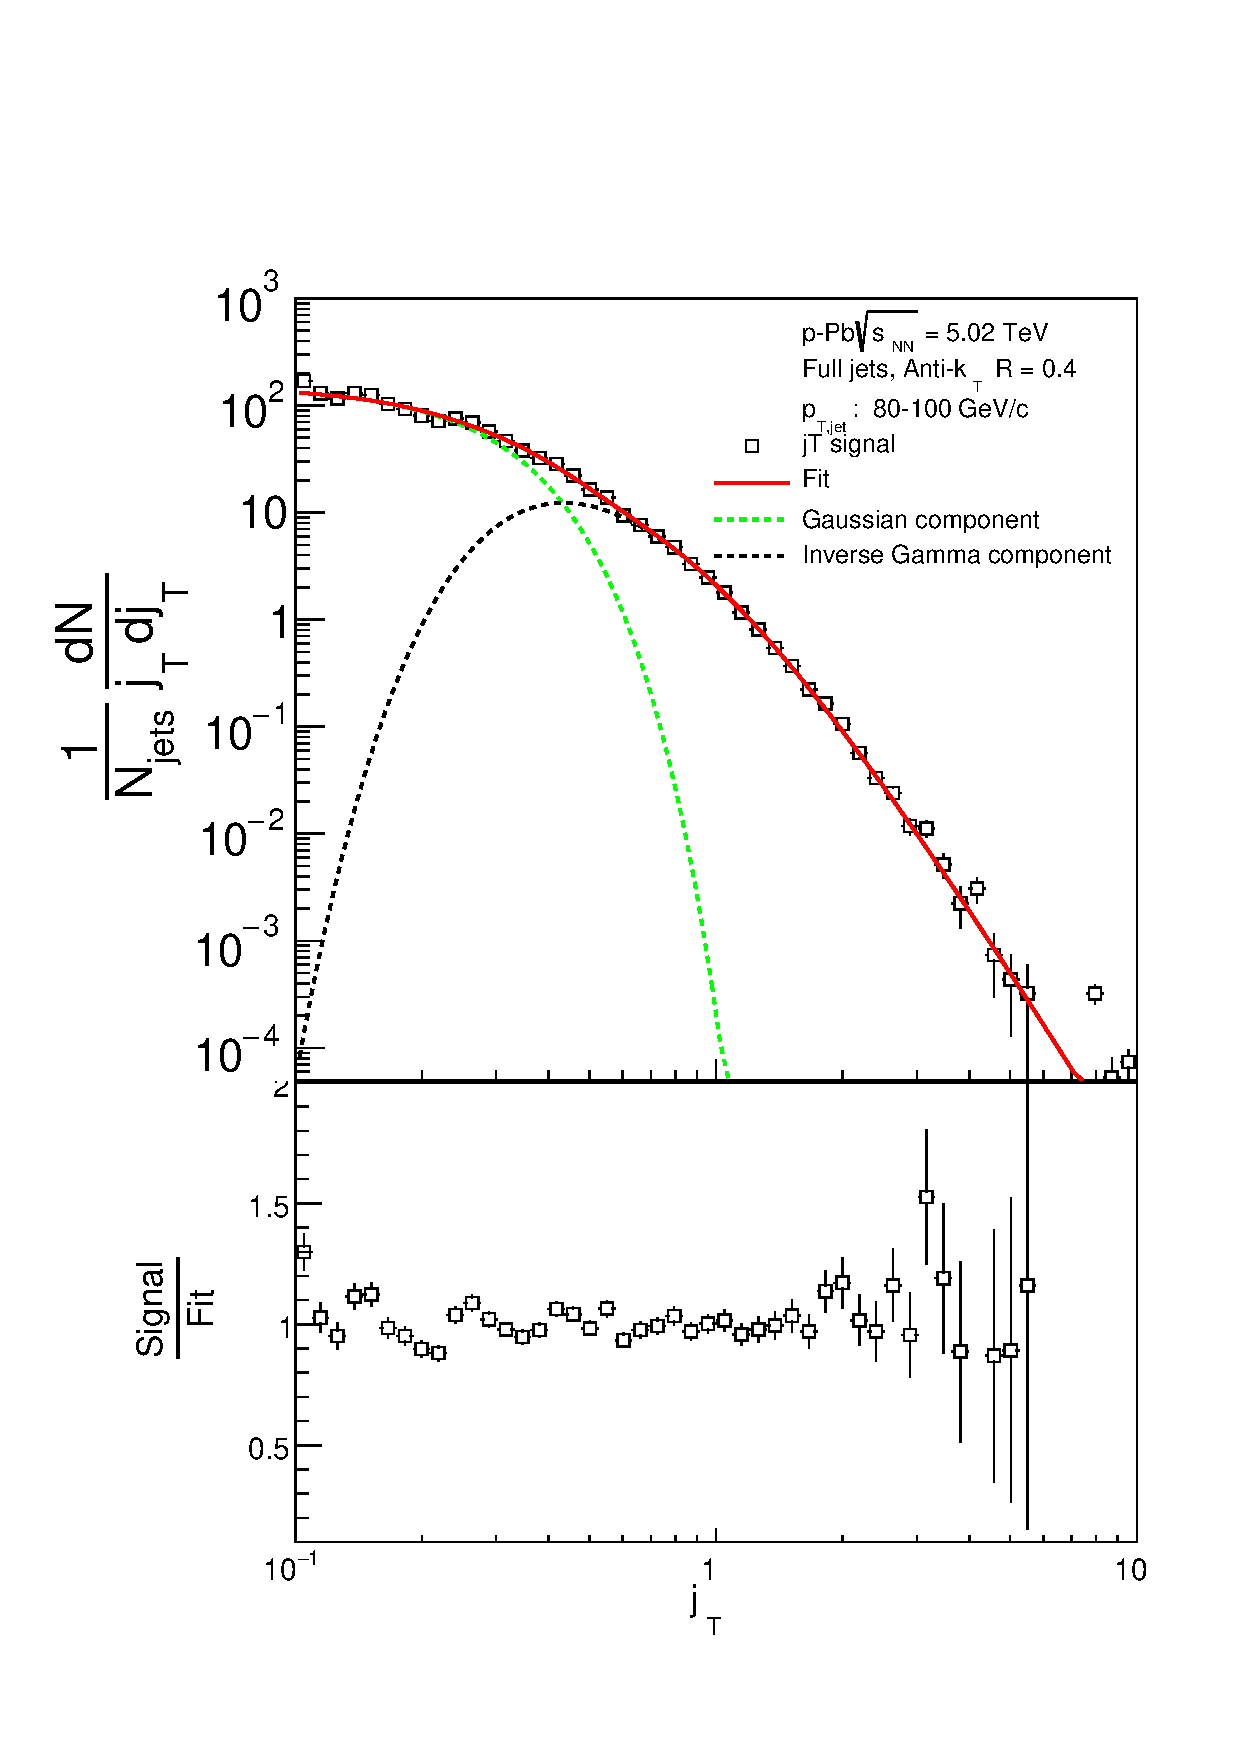
\includegraphics[width=0.95\textwidth]{results/JetConejTSignalFit/JetConejTSignalFitNFin00JetPt06randomBgBayes}
\end{subfigure}
\begin{subfigure}{0.24\textwidth}
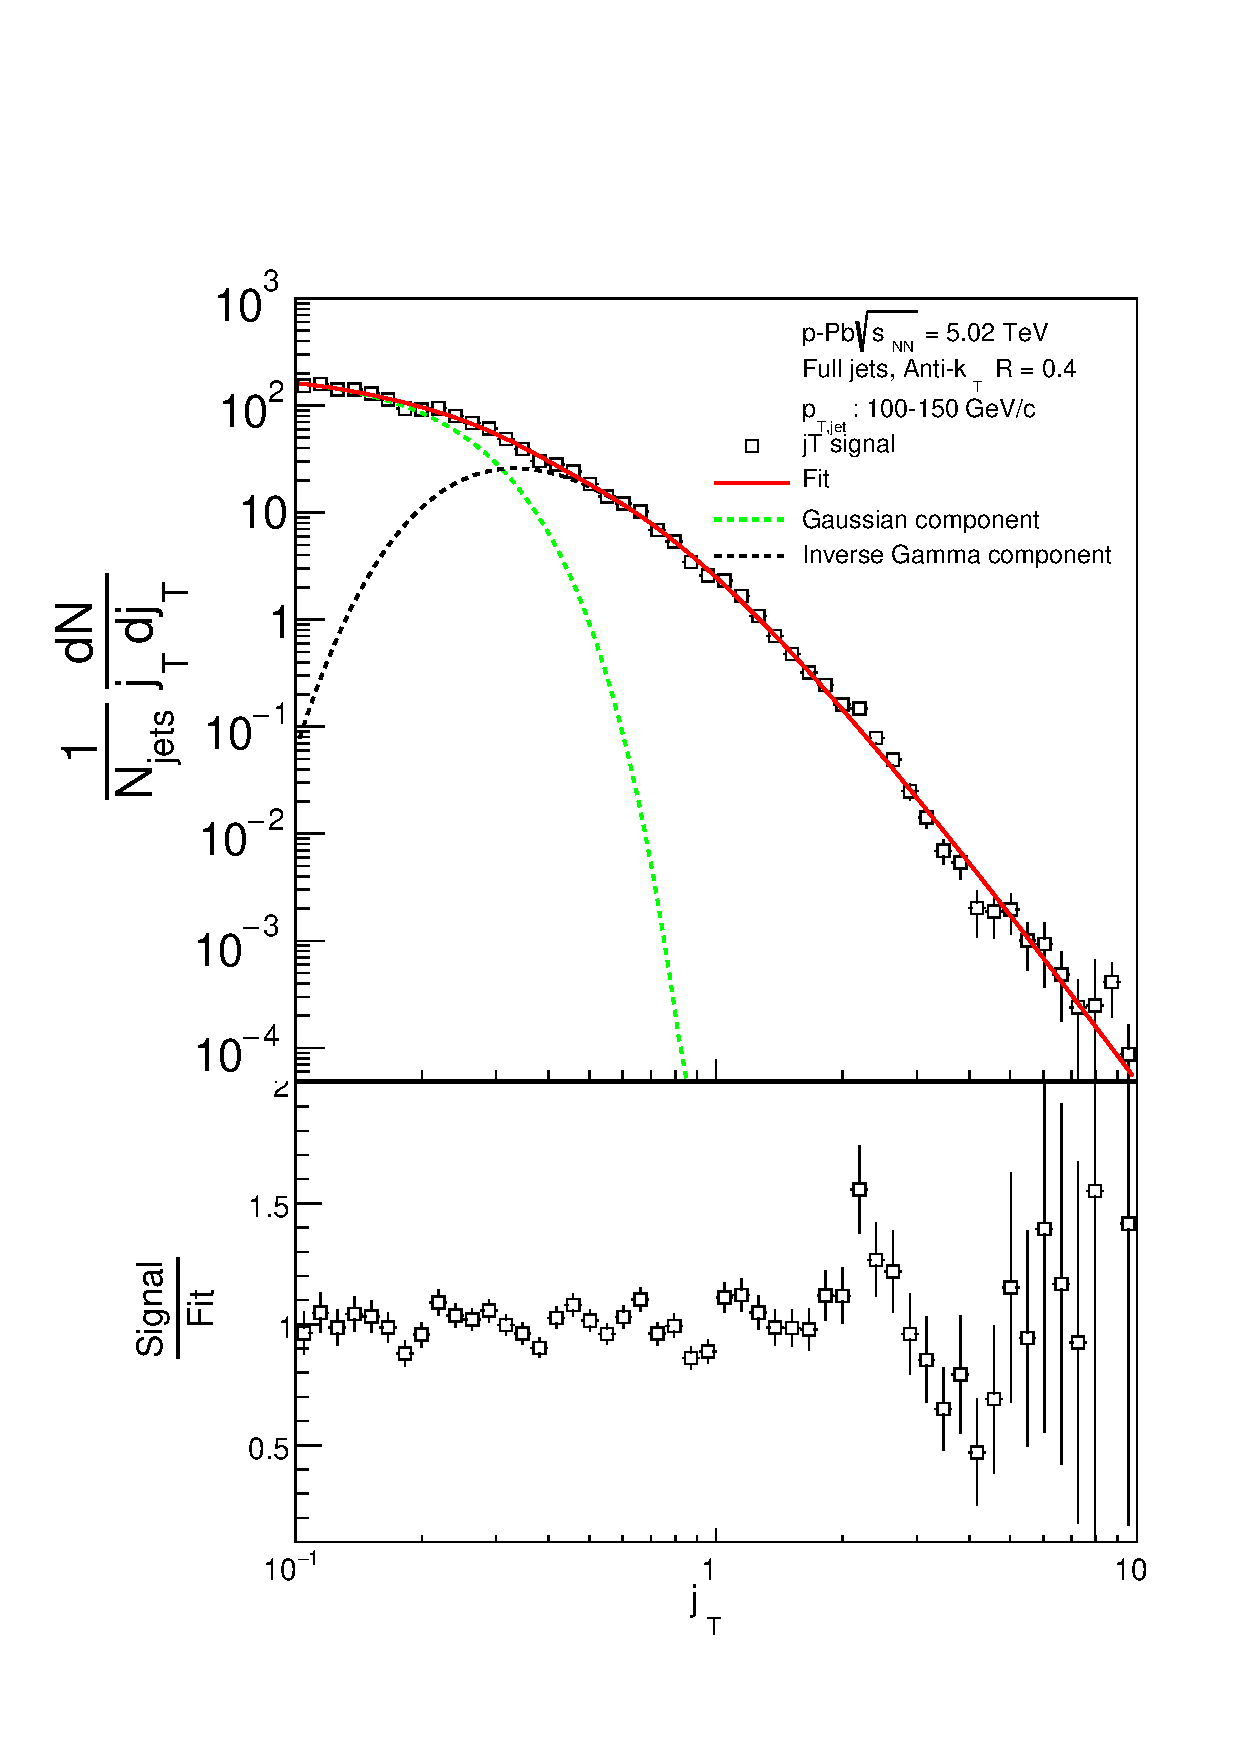
\includegraphics[width=0.95\textwidth]{results/JetConejTSignalFit/JetConejTSignalFitNFin00JetPt07randomBgBayes}
\end{subfigure}
\caption{$\jt{}$ signal with random bacgkround subtraction fits in different jet $\pt{}$ bins}
\label{fig:fitsrandombg}
\end{figure}

\begin{figure}
\centering
\begin{subfigure}{0.24\textwidth}
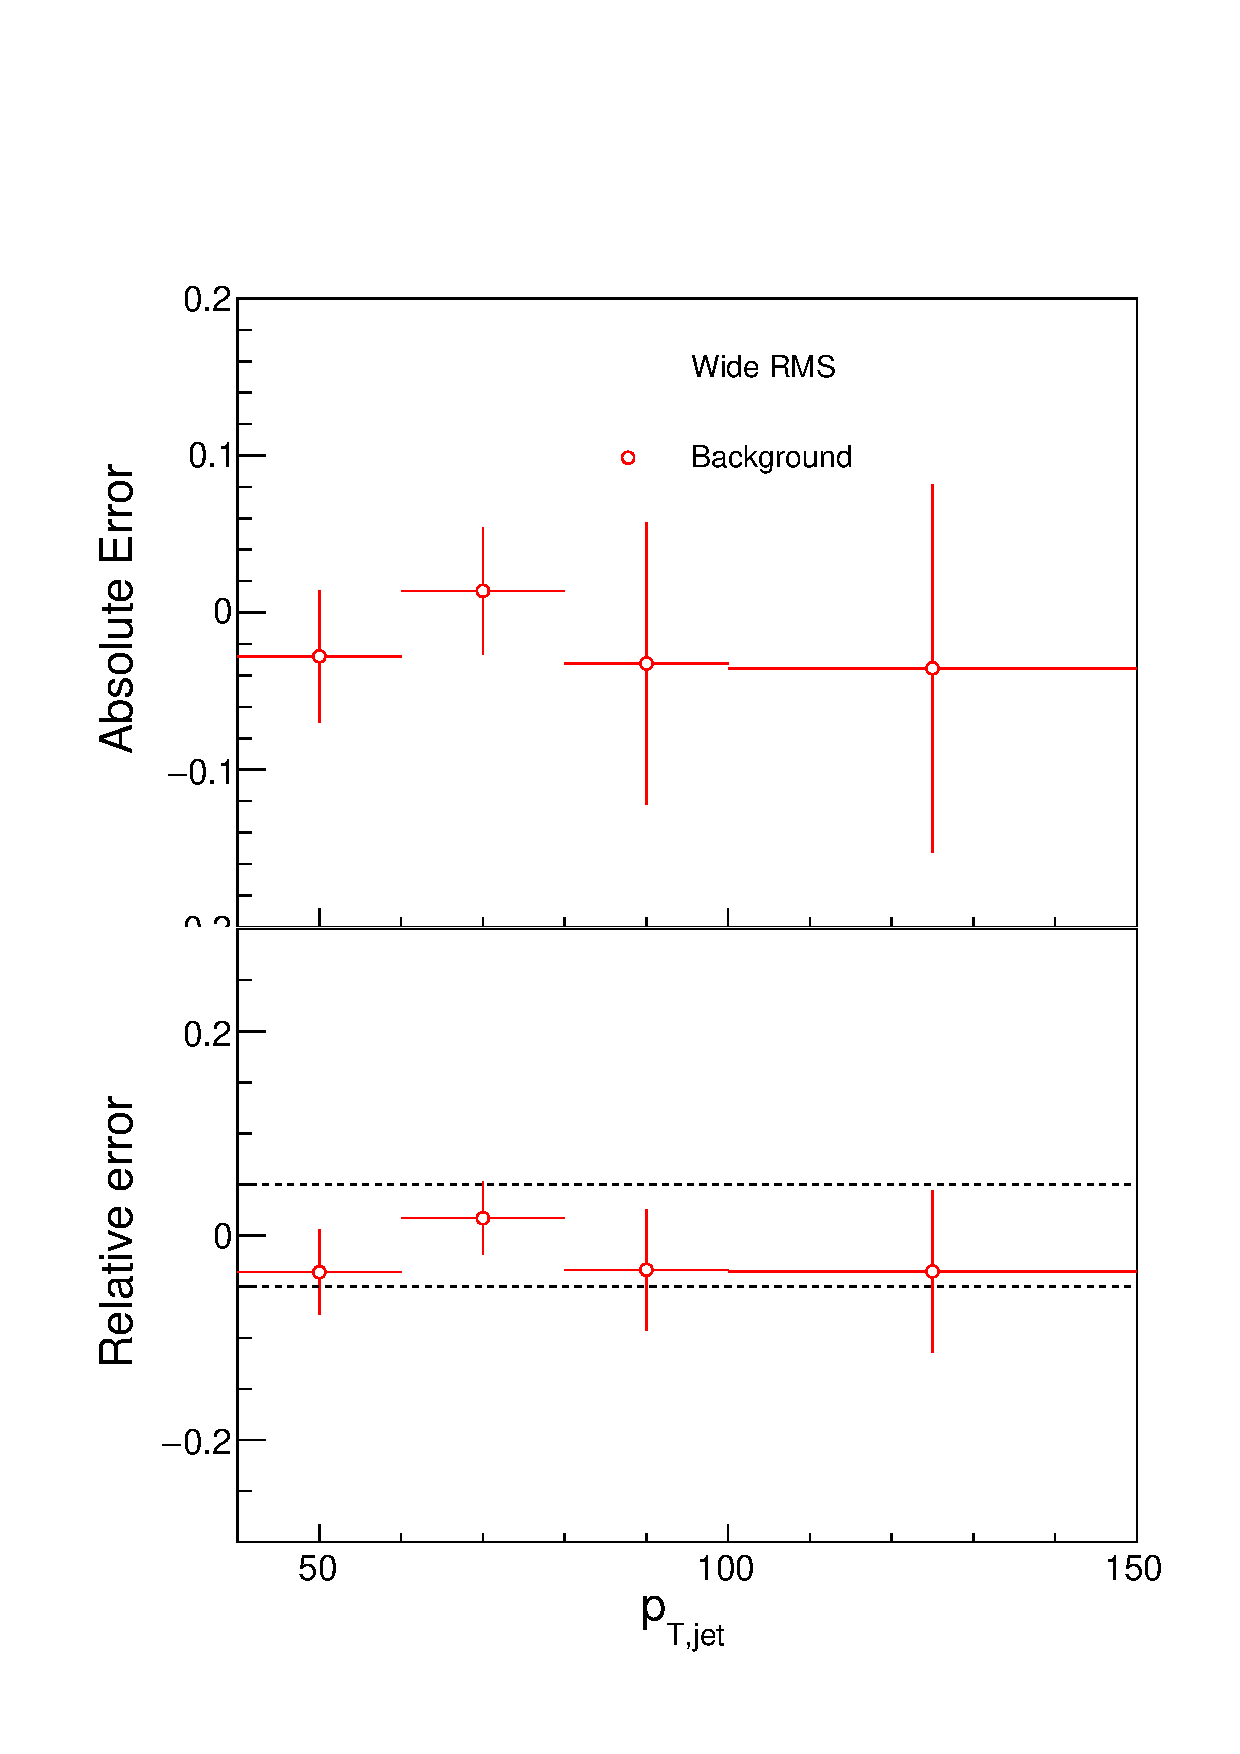
\includegraphics[width=0.95\textwidth]{results/SystematicErrors/SystematicErrorsGammaRMS_BgNFin00JetPt08_linx_data}
\end{subfigure}
\begin{subfigure}{0.24\textwidth}
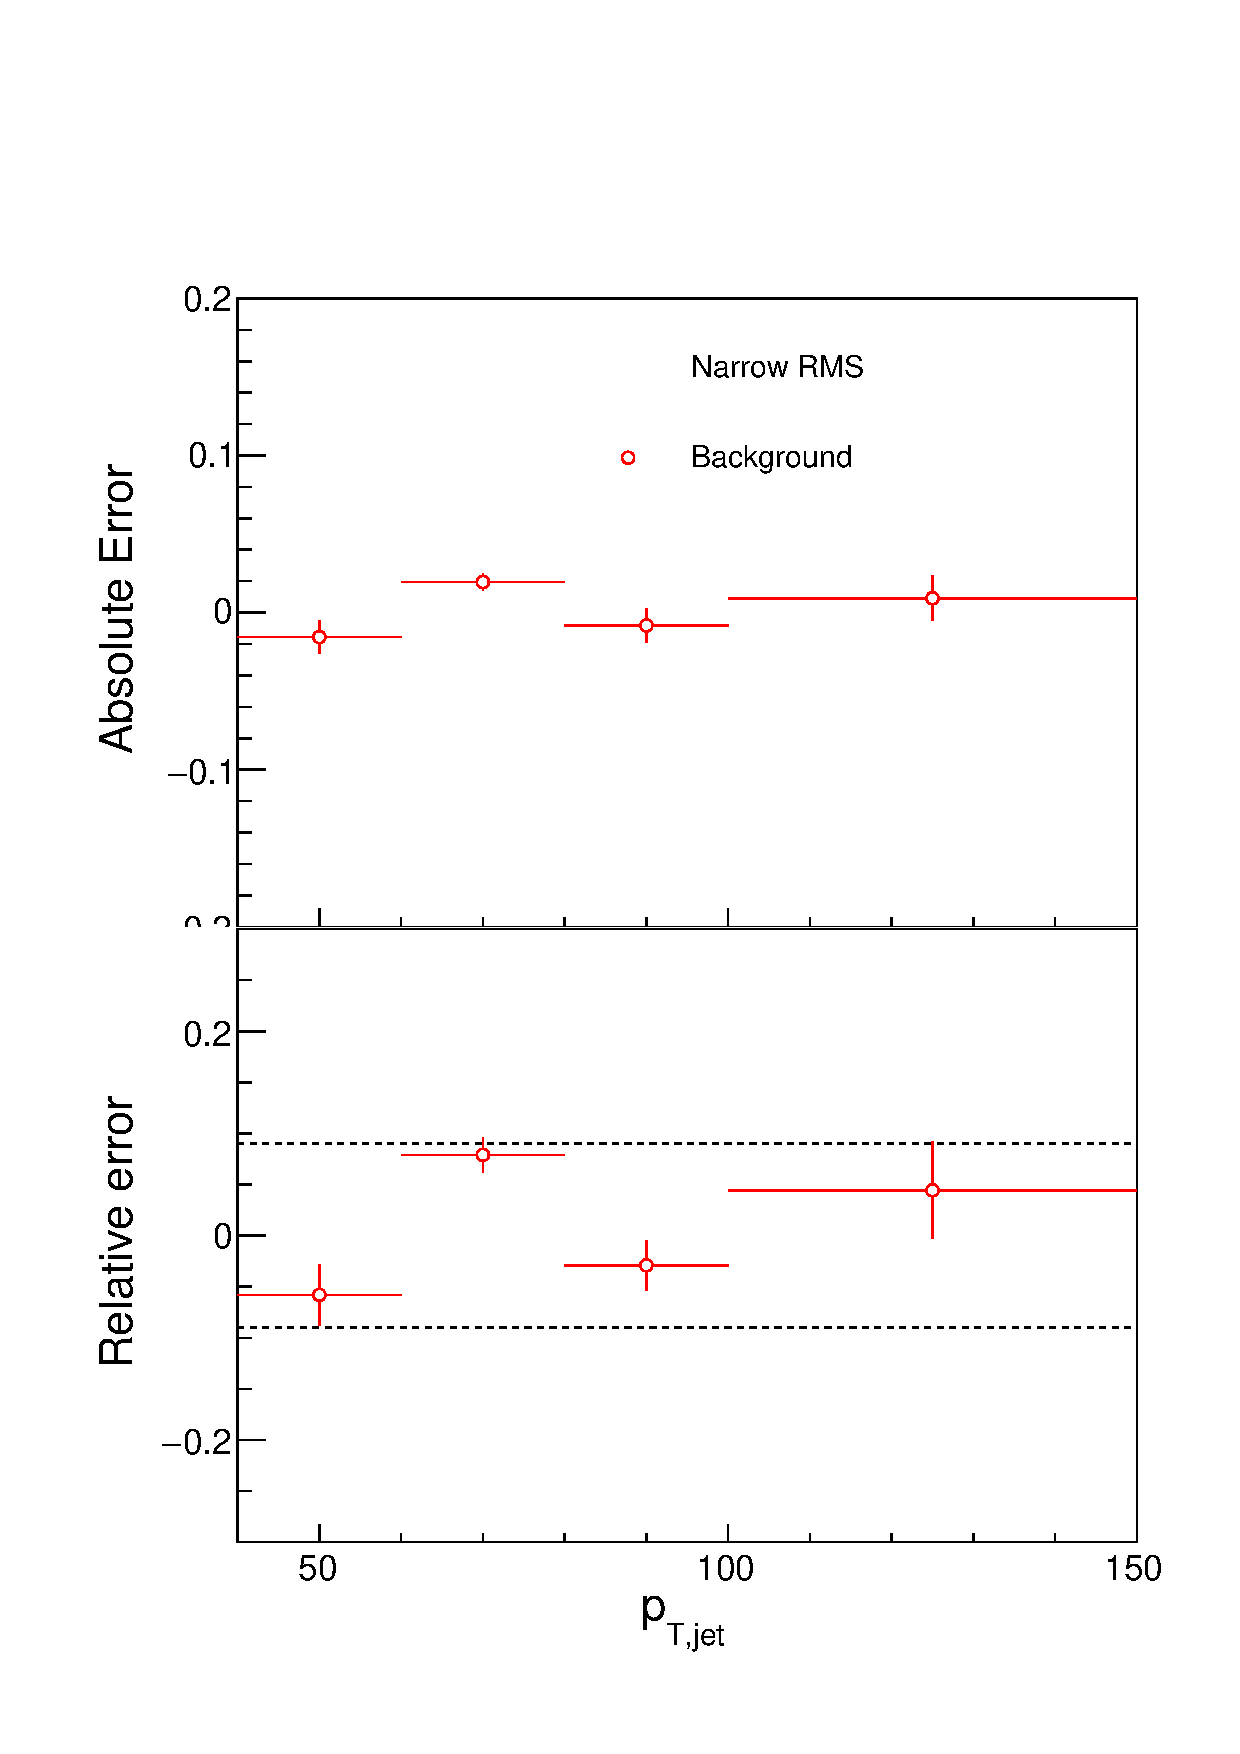
\includegraphics[width=0.95\textwidth]{results/SystematicErrors/SystematicErrorsGausRMS_BgNFin00JetPt08_linx_data}
\end{subfigure}
\caption{Differences between perpendicular cone and random background subtraction in the resulting RMS values.}
\label{fig:systbg}
\end{figure}

  
  
  
  \subsection{Unfolding}
Unfolding is performed using both SVD and Bayesian unfolding. Difference between the methods is taken as the systematic error. Since SVD unfolding does not have a 2 dimensional options, the unfolding is done bin by bin. The resulting distributions after SVD unfolding and background subtraction with the perpendicular cone method are shown in fig \ref{fig:fitsSVD}. Resulting differences between the methods for different components are shown in figure \ref{fig:systunf}.

\begin{figure}
\centering
\begin{subfigure}{0.24\textwidth}
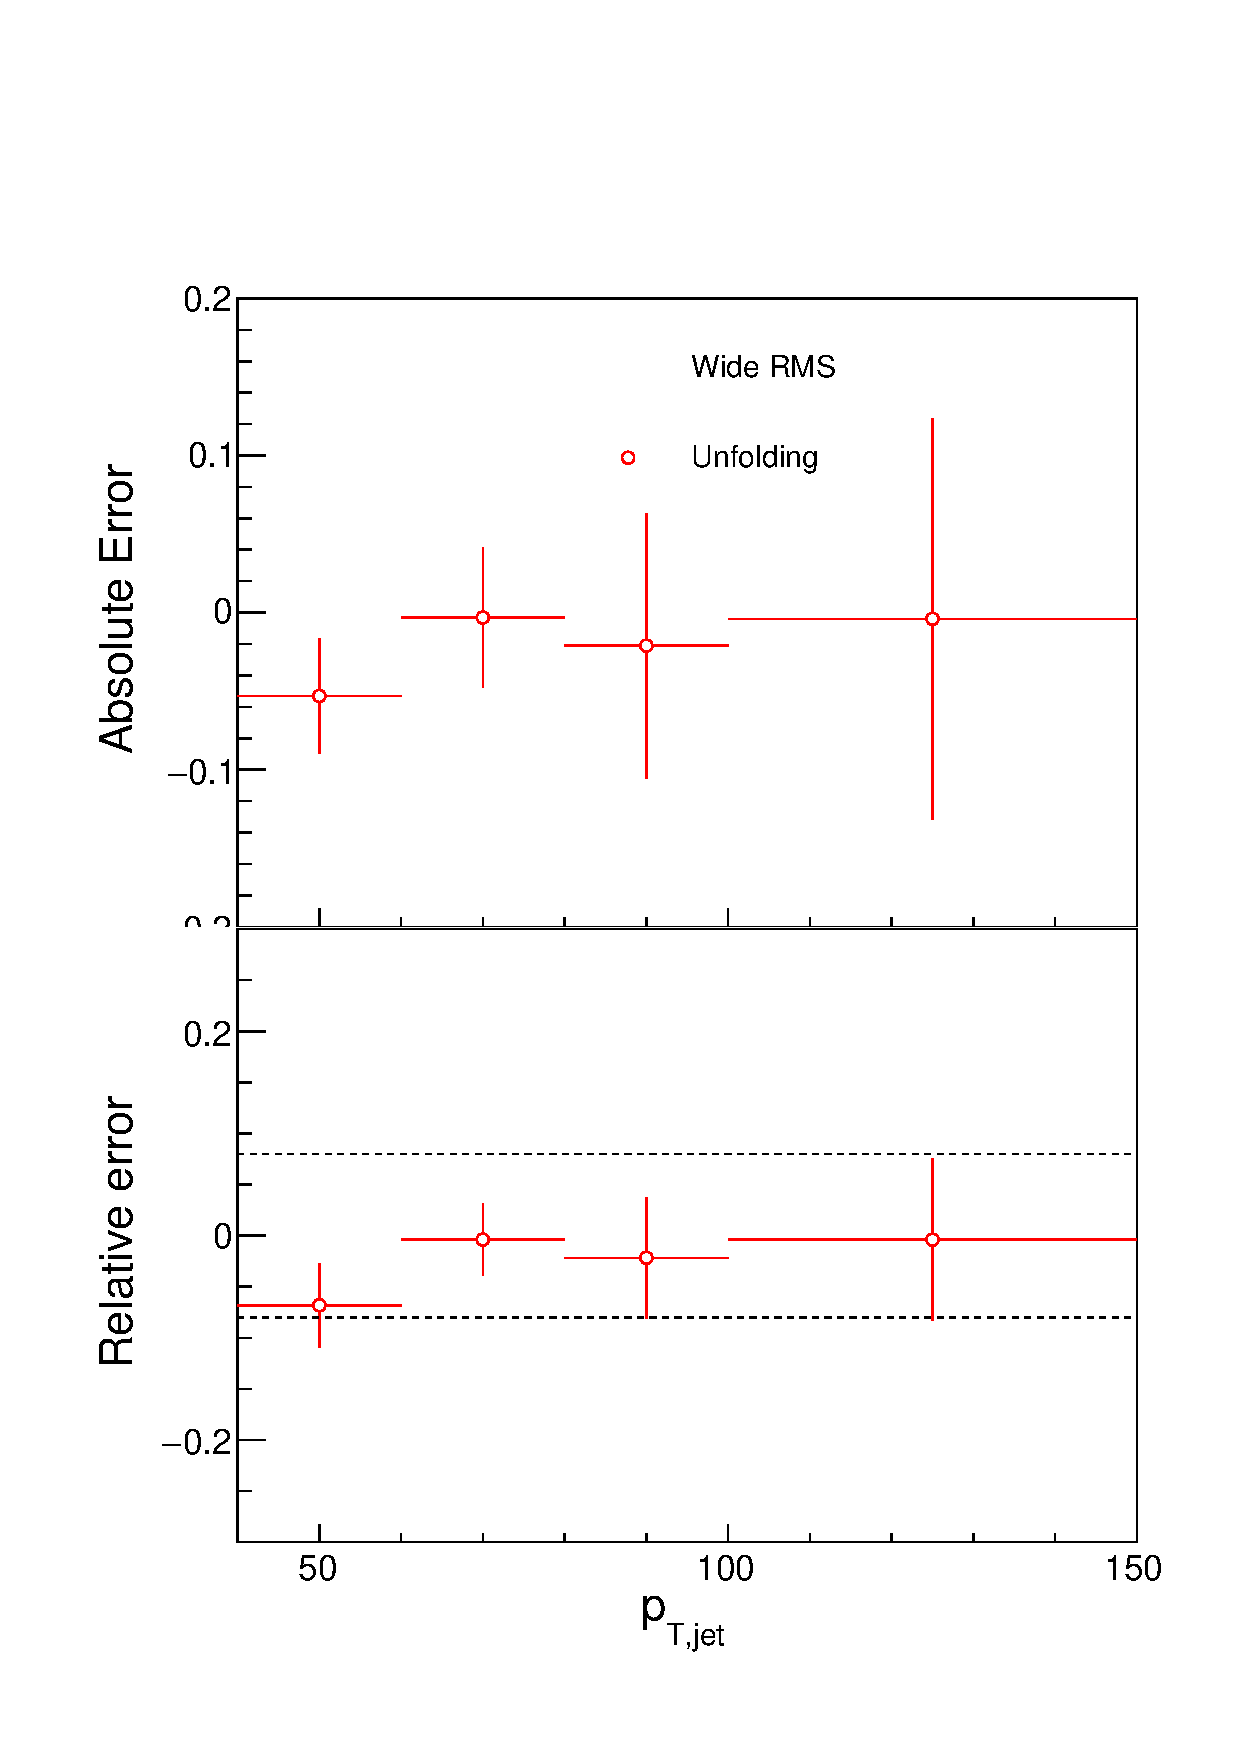
\includegraphics[width=0.95\textwidth]{results/SystematicErrors/SystematicErrorsGammaRMS_UnfNFin00JetPt08_linx_data}
\end{subfigure}
\begin{subfigure}{0.24\textwidth}
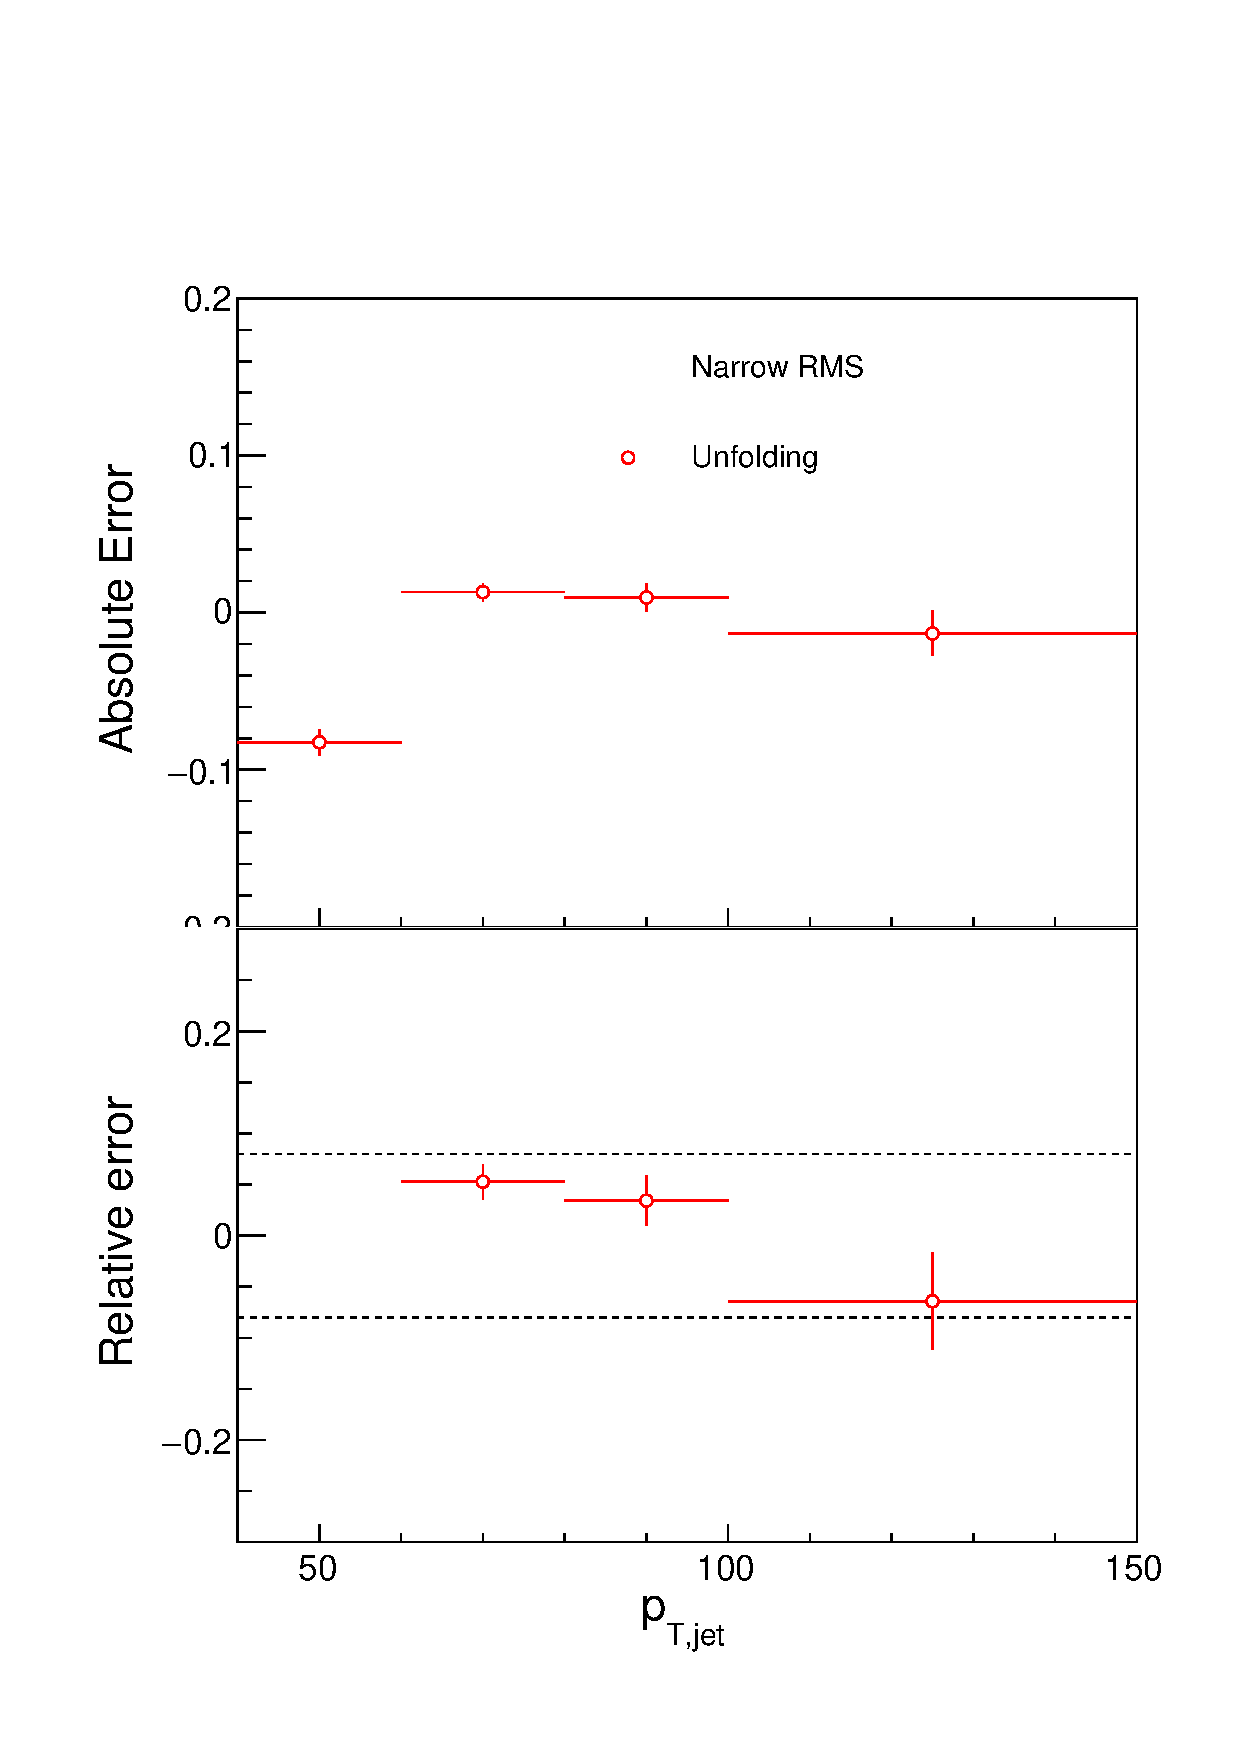
\includegraphics[width=0.95\textwidth]{results/SystematicErrors/SystematicErrorsGausRMS_UnfNFin00JetPt08_linx_data}
\end{subfigure}
\caption{Differences between Bayesian and SVD unfolding in the resulting RMS values}
\label{fig:systunf}
\end{figure}

  
\subsubsection{Effect of number of iterations}
\label{sec:iterations}
The iterative unfolding algorithm permits the change of number of iterations. The unfolding was carried out using different numbers of iterations. The results from these different cases are shown in Fig.~\ref{fig:iterations}. The results are compared to the default unfolding algorithm with 4 iterations. The difference in results between the different cases is mostly less than 2.5\%.
\begin{figure}
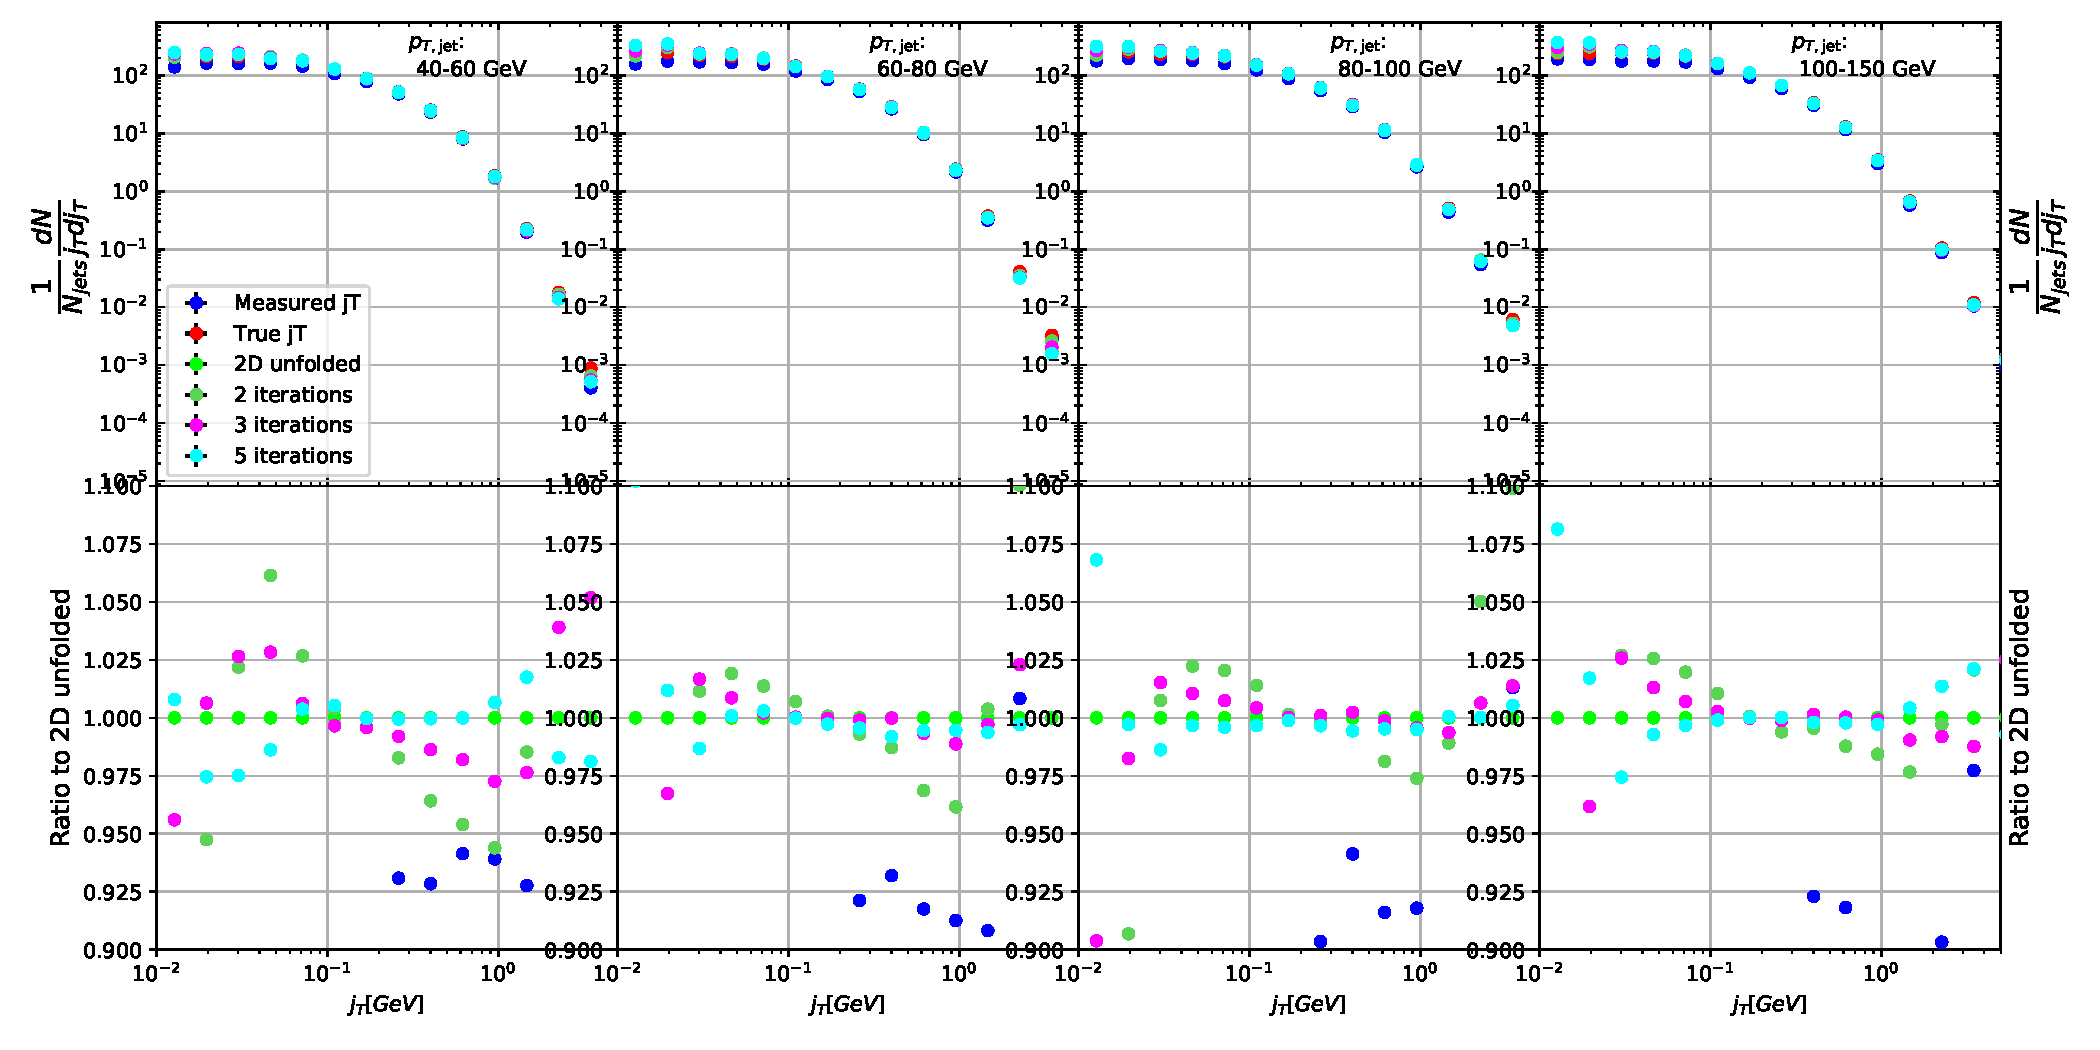
\includegraphics[width=0.99\textwidth]{figures/systematics/IterationsComparison.pdf}
\caption{Unfolding with different number of iterations}
\label{fig:iterations}
\end{figure}

\subsubsection{Effect of different prior}
\label{sec:prior}
The iterative algorithm requires a prior estimate of the shape of the distribution. As a default prior the truth (particle level) distribution is used. To test the effect of changing the prior we instead use the unfolded $\jt{}$ distribution as prior. The results are compared to the unfolding algorithm with the default prior. This is shown in Fig.~\ref{fig:prior} The difference in results between the different cases is mostly less than 2.5\%. 
\begin{figure}
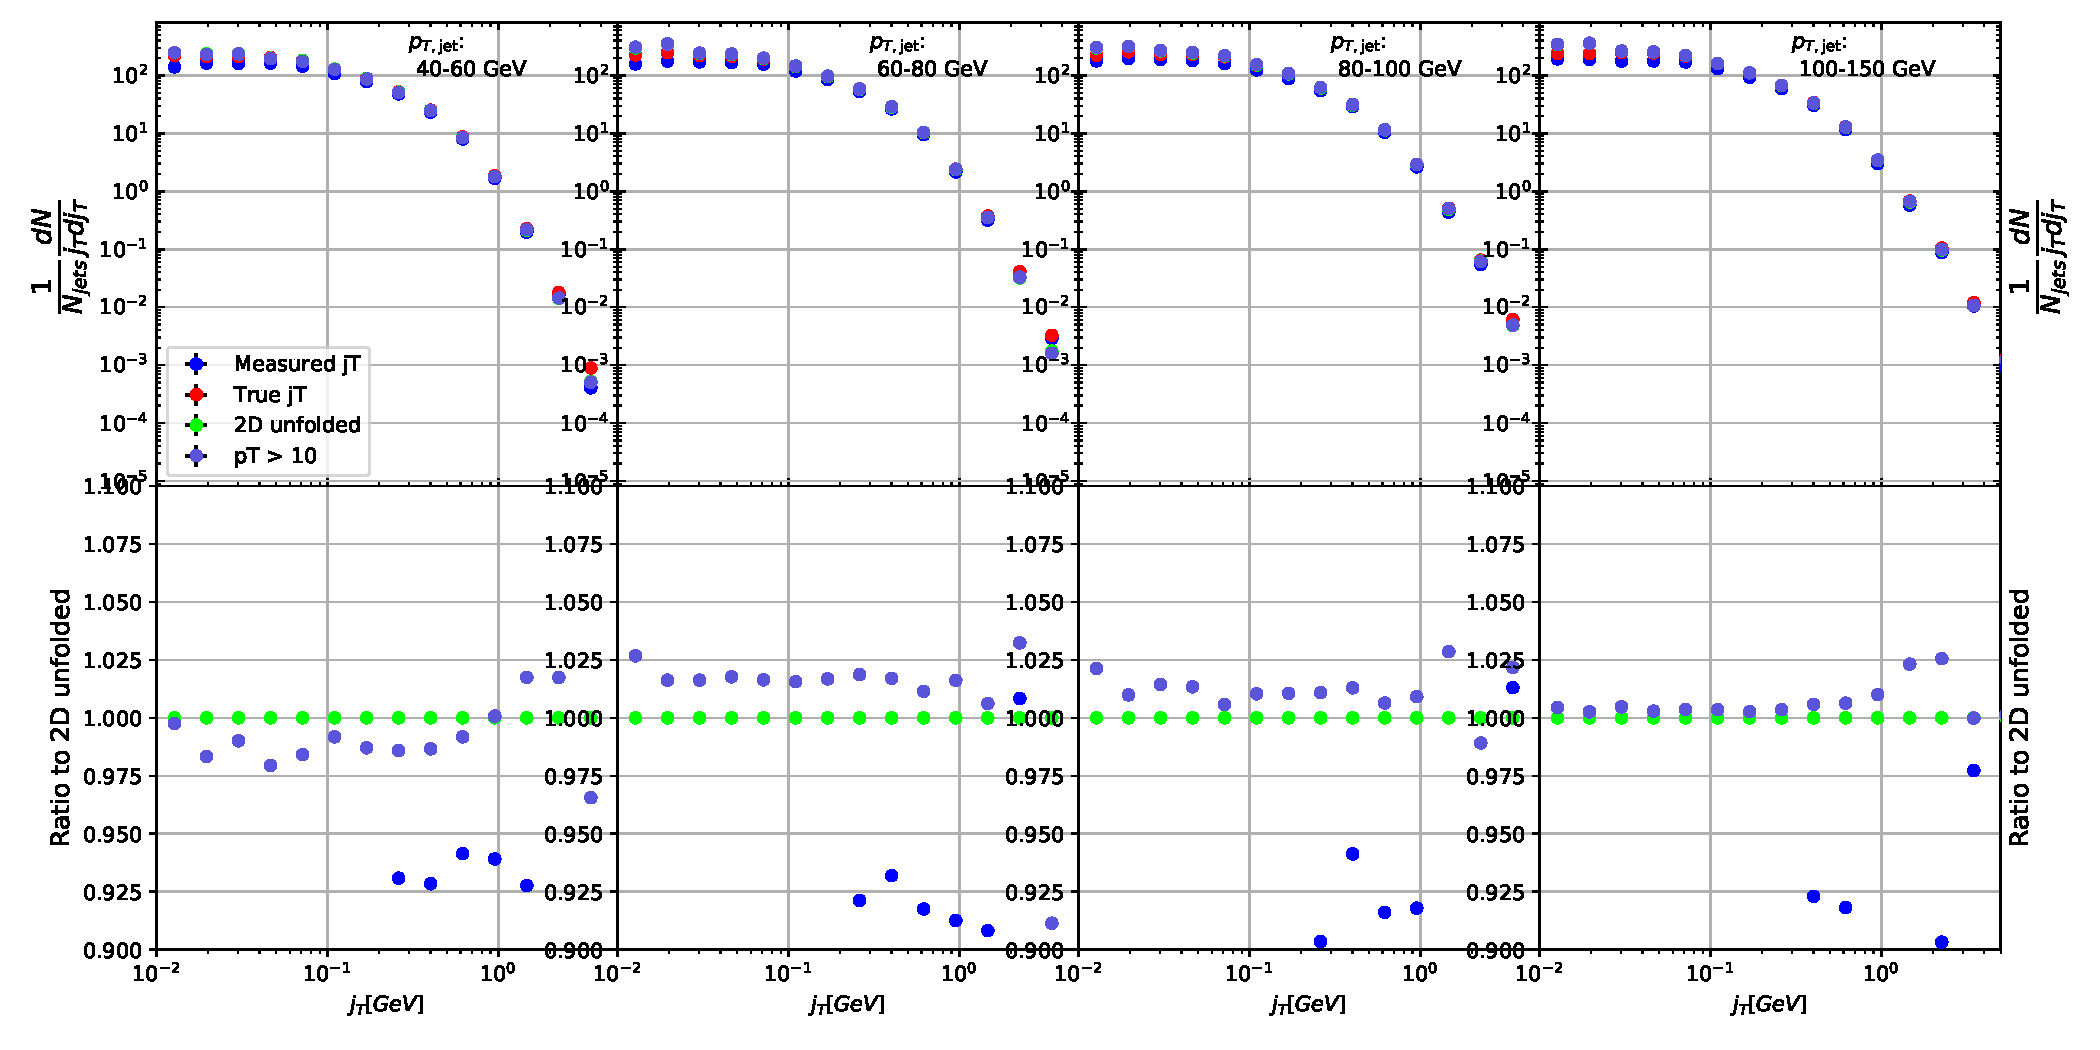
\includegraphics[width=0.99\textwidth]{figures/systematics/PtCutComparison10.pdf}
\caption{Effect of changing minimum jet $\pt{}$ used in unfolding from 5 to 10 \gev}
\label{fig:prior}
\end{figure}

\subsubsection{Effect of $\pt{}$ truncation}
\label{sec:truncation}
As an additional check the unfolding is carried out with different $\pt{jet}$ truncation values. By default the full range of $\pt{jet} > 5 \gev$ is used. As an option the we test the unfolding by only using the response matrix for $\pt{jet} > 10 \gev$. The results of this test are shown in Fig.~\ref{fig:truncation}

\begin{figure}
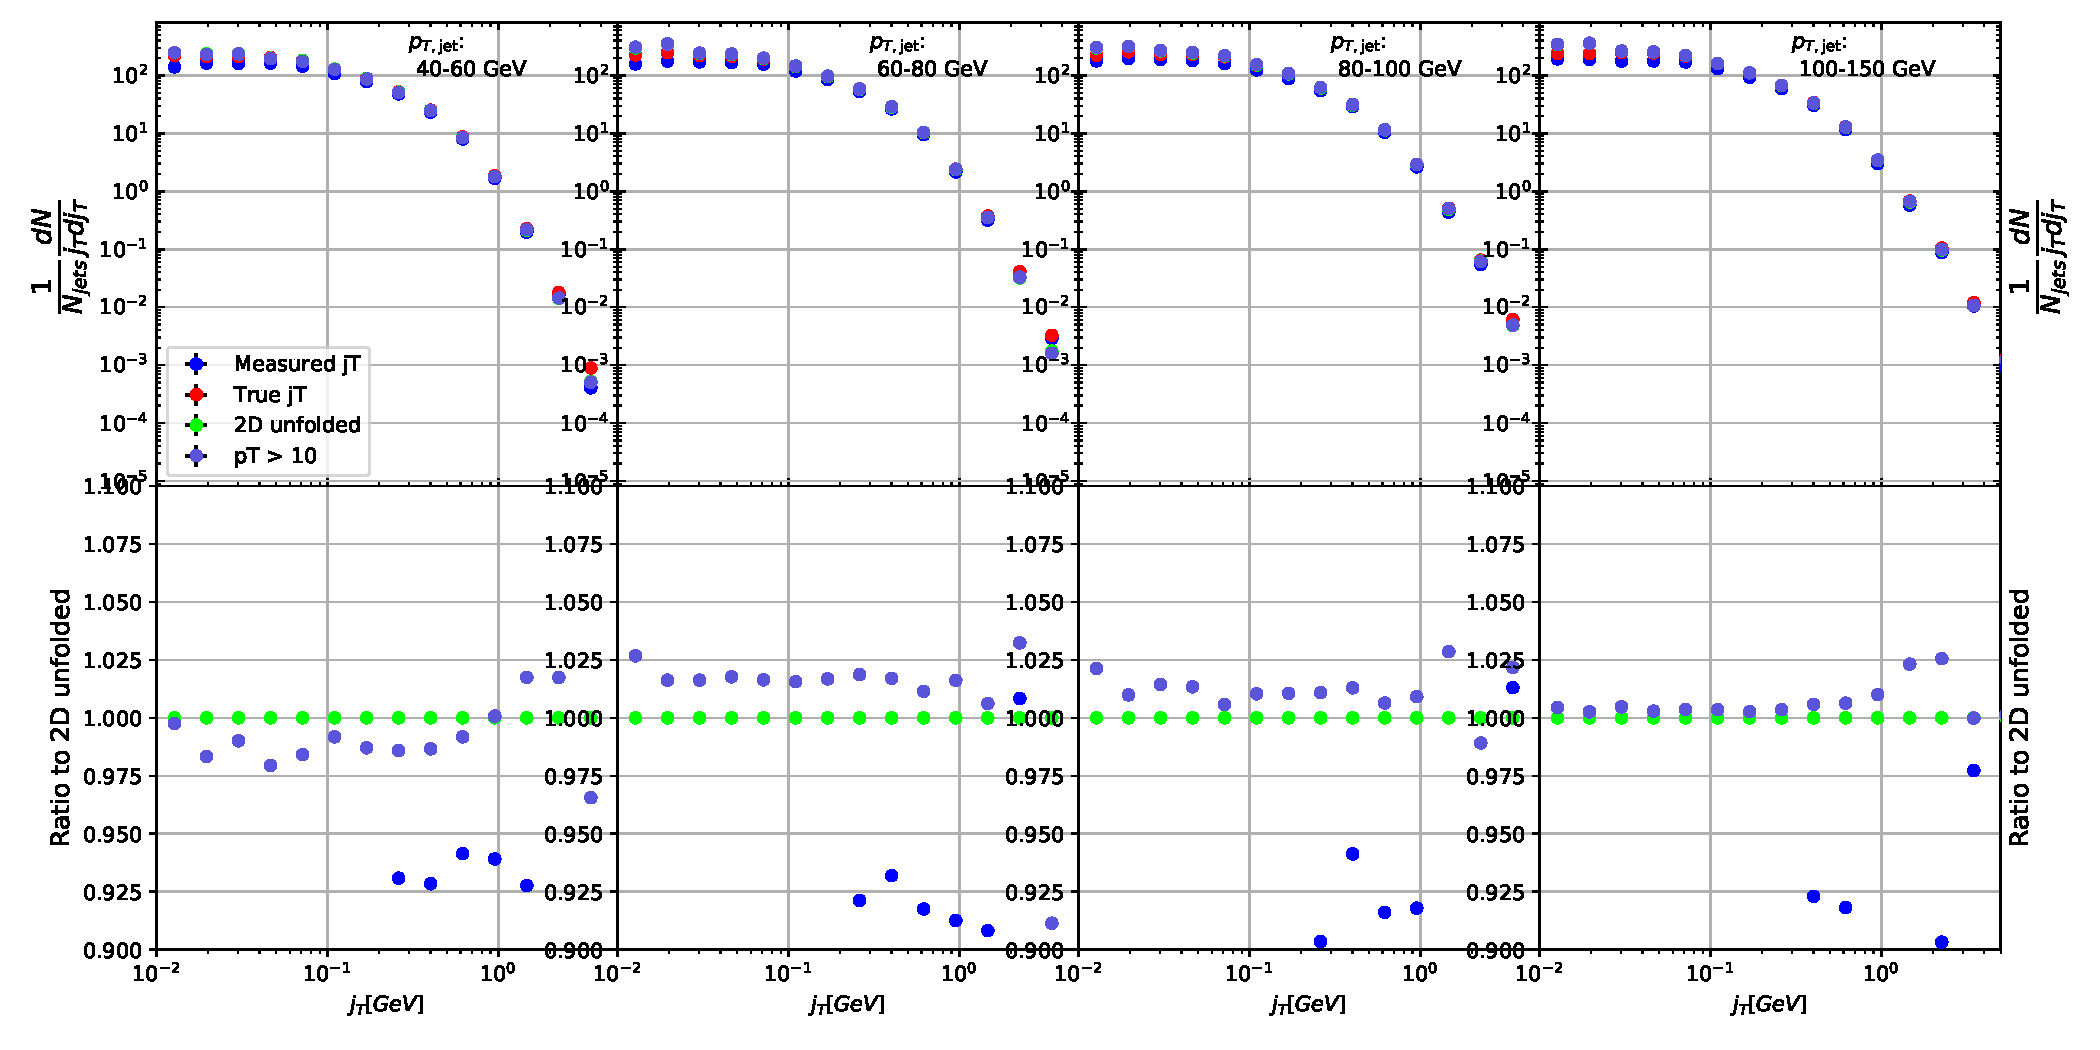
\includegraphics[width=0.99\textwidth]{figures/systematics/PtCutComparison10.pdf}
\caption{Effect of changing minimum jet $\pt{}$ used in unfolding from 5 to 10 \gev}
\label{fig:truncation}
\end{figure}


  
  
  \subsection{Tracking}
 Systematic effects originating from uncertainty in the tracking efficiency are estimated through a \pythia~simulation, where an artificial inefficiency of 3\% is introduced. i.e. 3 \% of tracks are randomly removed from each event. 
  \subsection{EMCAL}
  The analysis uses EMCAL clusters only in the reconstruction of jets. Thus the only way uncertainty in EMCAL performance can affect the results is through modification of jet momentum or axis.
  
  Uncertainty related to the EMCAL energy scale was estimated by scaling cluster energies up and down by 2 \% in a PYTHIA particle level simulation. Similarly the jet momentum was scaled by $\pm 2\%$ when determining the jet $\pt{}$ bin. In the analysis EMCAL is used only in jet reconstruction, not for calculating $\jt{}$. The only ways EMCAL uncertainty can affect the analysis are changes in jet energy and jet axis. Jet axis shouldn't significantly change, so the main contribution should be changes in jet $\pt{}$ bin.

The results are shown in Fig.~\ref{fig:systemcal}. The resulting systematic uncertainties are shown in Fig.~\ref{fig:systemcal2}. The uncertainty is taken to be 1\%. 

\begin{figure}
\centering
\begin{subfigure}{0.90\textwidth}
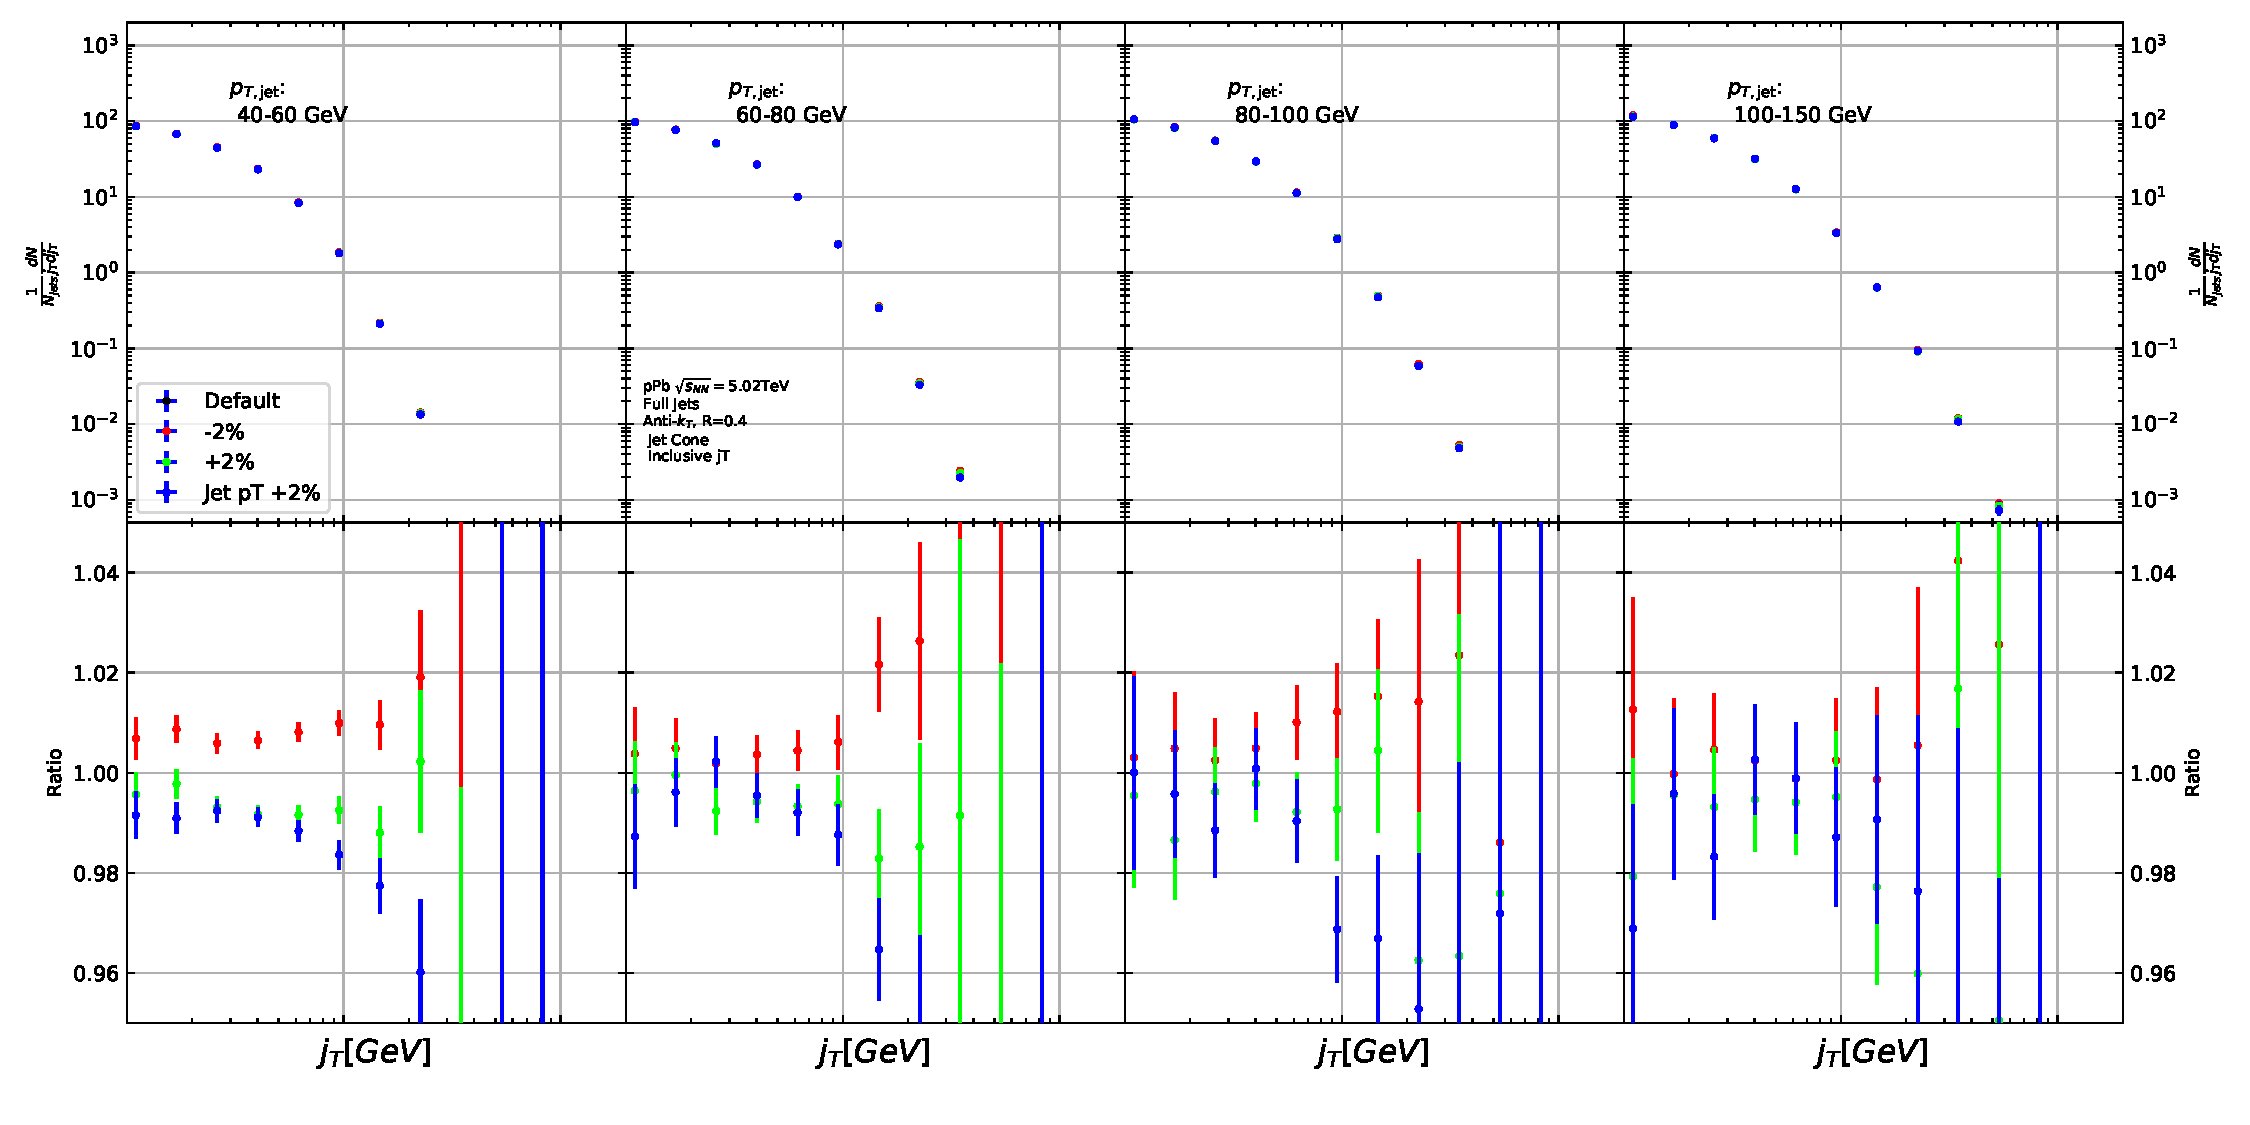
\includegraphics[width=0.95\textwidth]{figures/systematics/HadCorrComparisonJetPt4To8.pdf}
\end{subfigure}
%\begin{subfigure}{0.24\textwidth}
%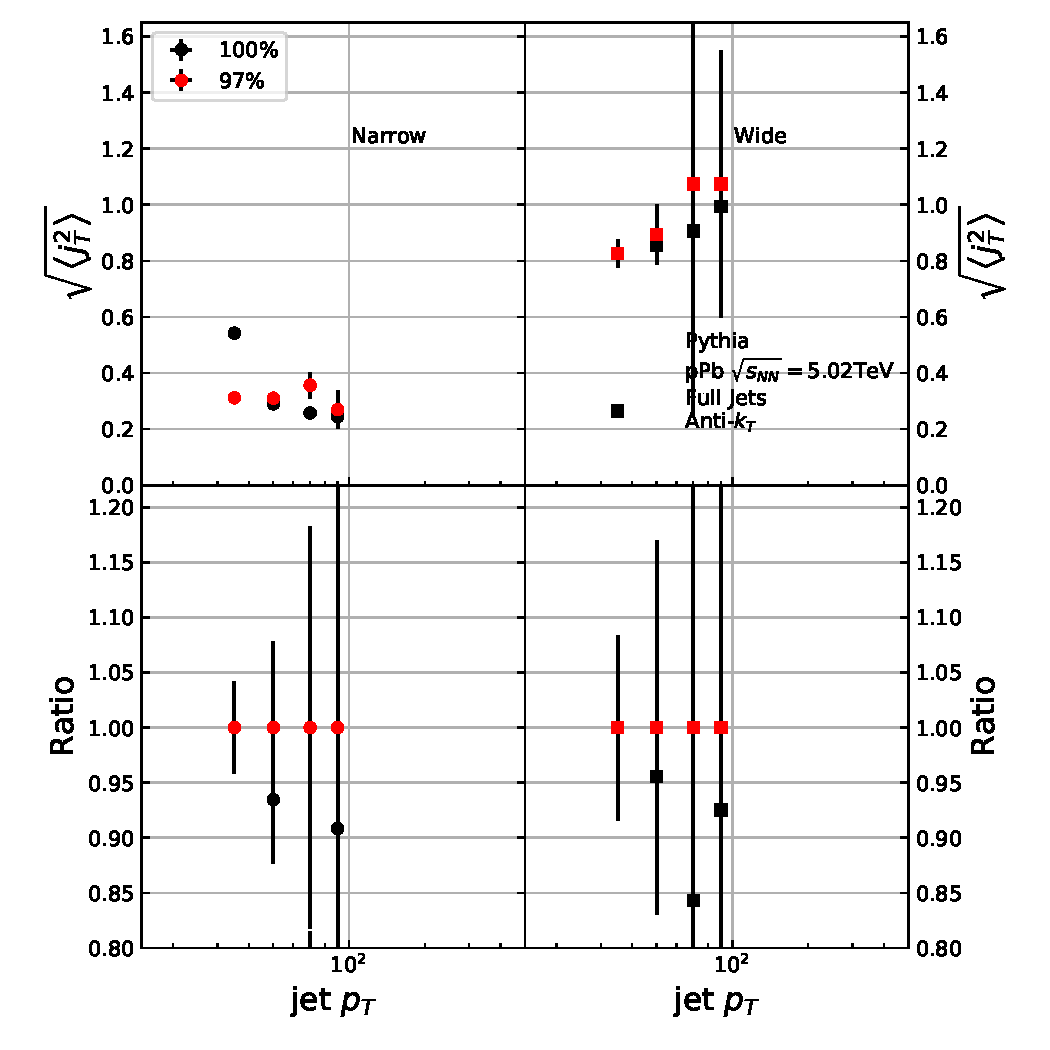
\includegraphics[width=0.95\textwidth]{RooUnfold/PythonFigures/TrackingSystematicsRMS.pdf}
%\end{subfigure}
\caption{Results from PYTHIA simulations with Cluster energies scale up/down by 2 \%. Additionally jet momenta were scaled by 2 \% when determining the jet $\pt{}$ bin.}
\label{fig:systemcal}
\end{figure}

\begin{figure}
\centering
\begin{subfigure}{0.45\textwidth}
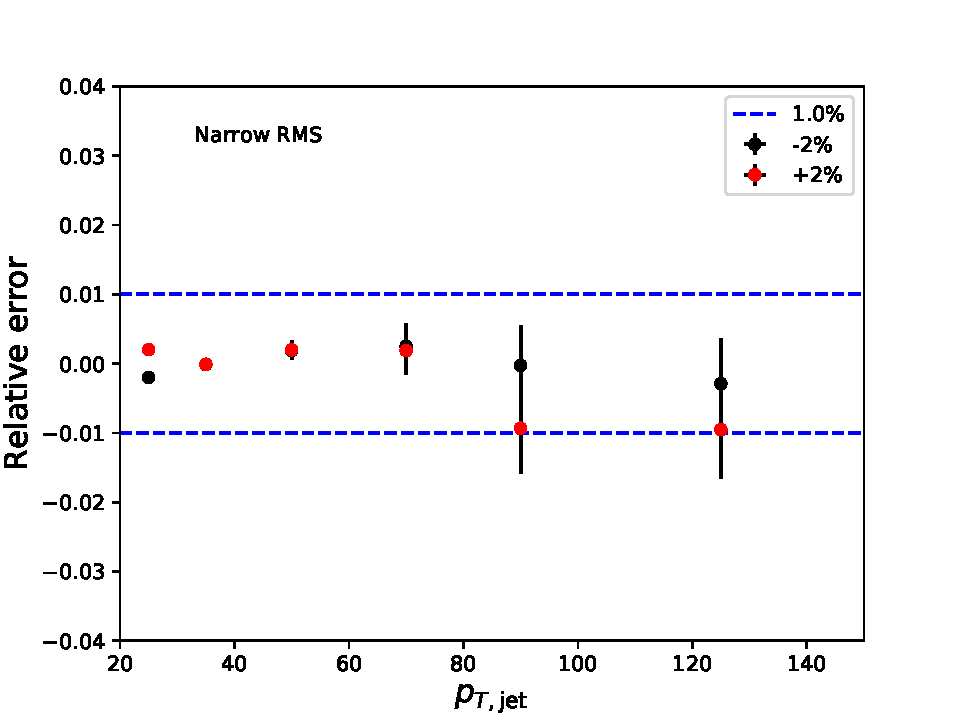
\includegraphics[width=0.95\textwidth]{figures/systematics/SystematicErrorsGausRMS_Emcal.pdf}
\end{subfigure}
\begin{subfigure}{0.45\textwidth}
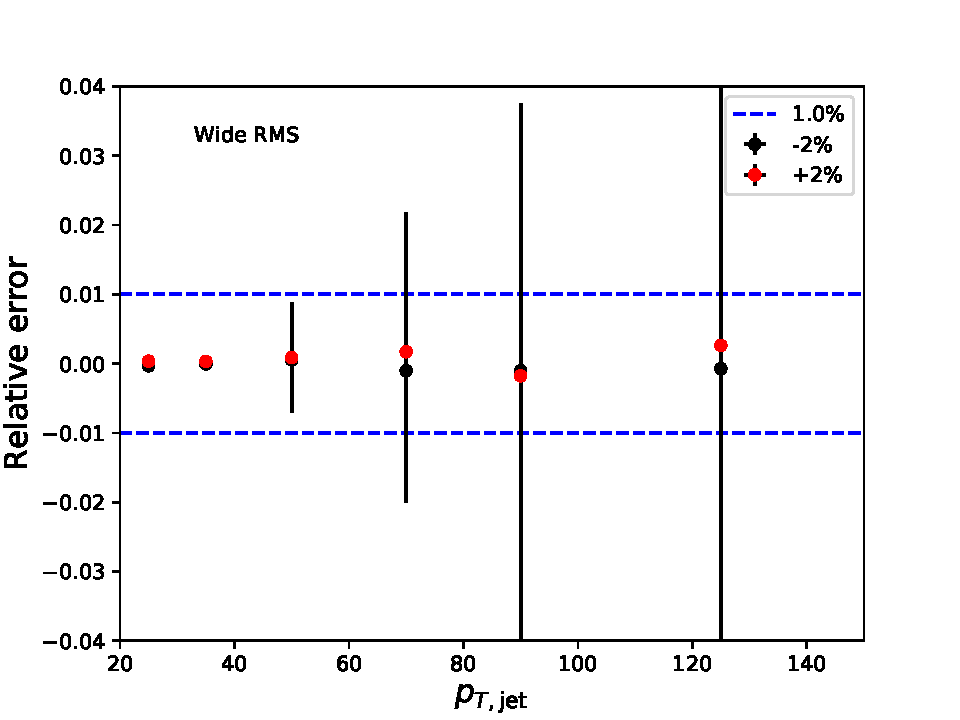
\includegraphics[width=0.95\textwidth]{figures/systematics/SystematicErrorsGammaRMS_Emcal.pdf}
\end{subfigure}
\caption{Relative systematic errors resulting from cluster energy uncertainty.}
\label{fig:systemcal2}
\end{figure}

  \subsection{Summary}

There is no tracking and no unfolding uncertainty in the Monte Carlo simulations. 



\subsection{Comparison between A and C side}
In 2013 there were issues with tracking. To rule out effects on $\jt{}$ distributions a study was performed comparing $\jt{}$ distributions between A and C side. {\color{red}Which is lead going side and which is proton going} No systematic differences were observed. Figure~\ref{fig:signalbg} shows the comparison between inclusive distributions between the different sides, both for minimum bias and EMCAL triggered datasets.

\begin{figure}
\centering
\begin{subfigure}{0.95\textwidth}
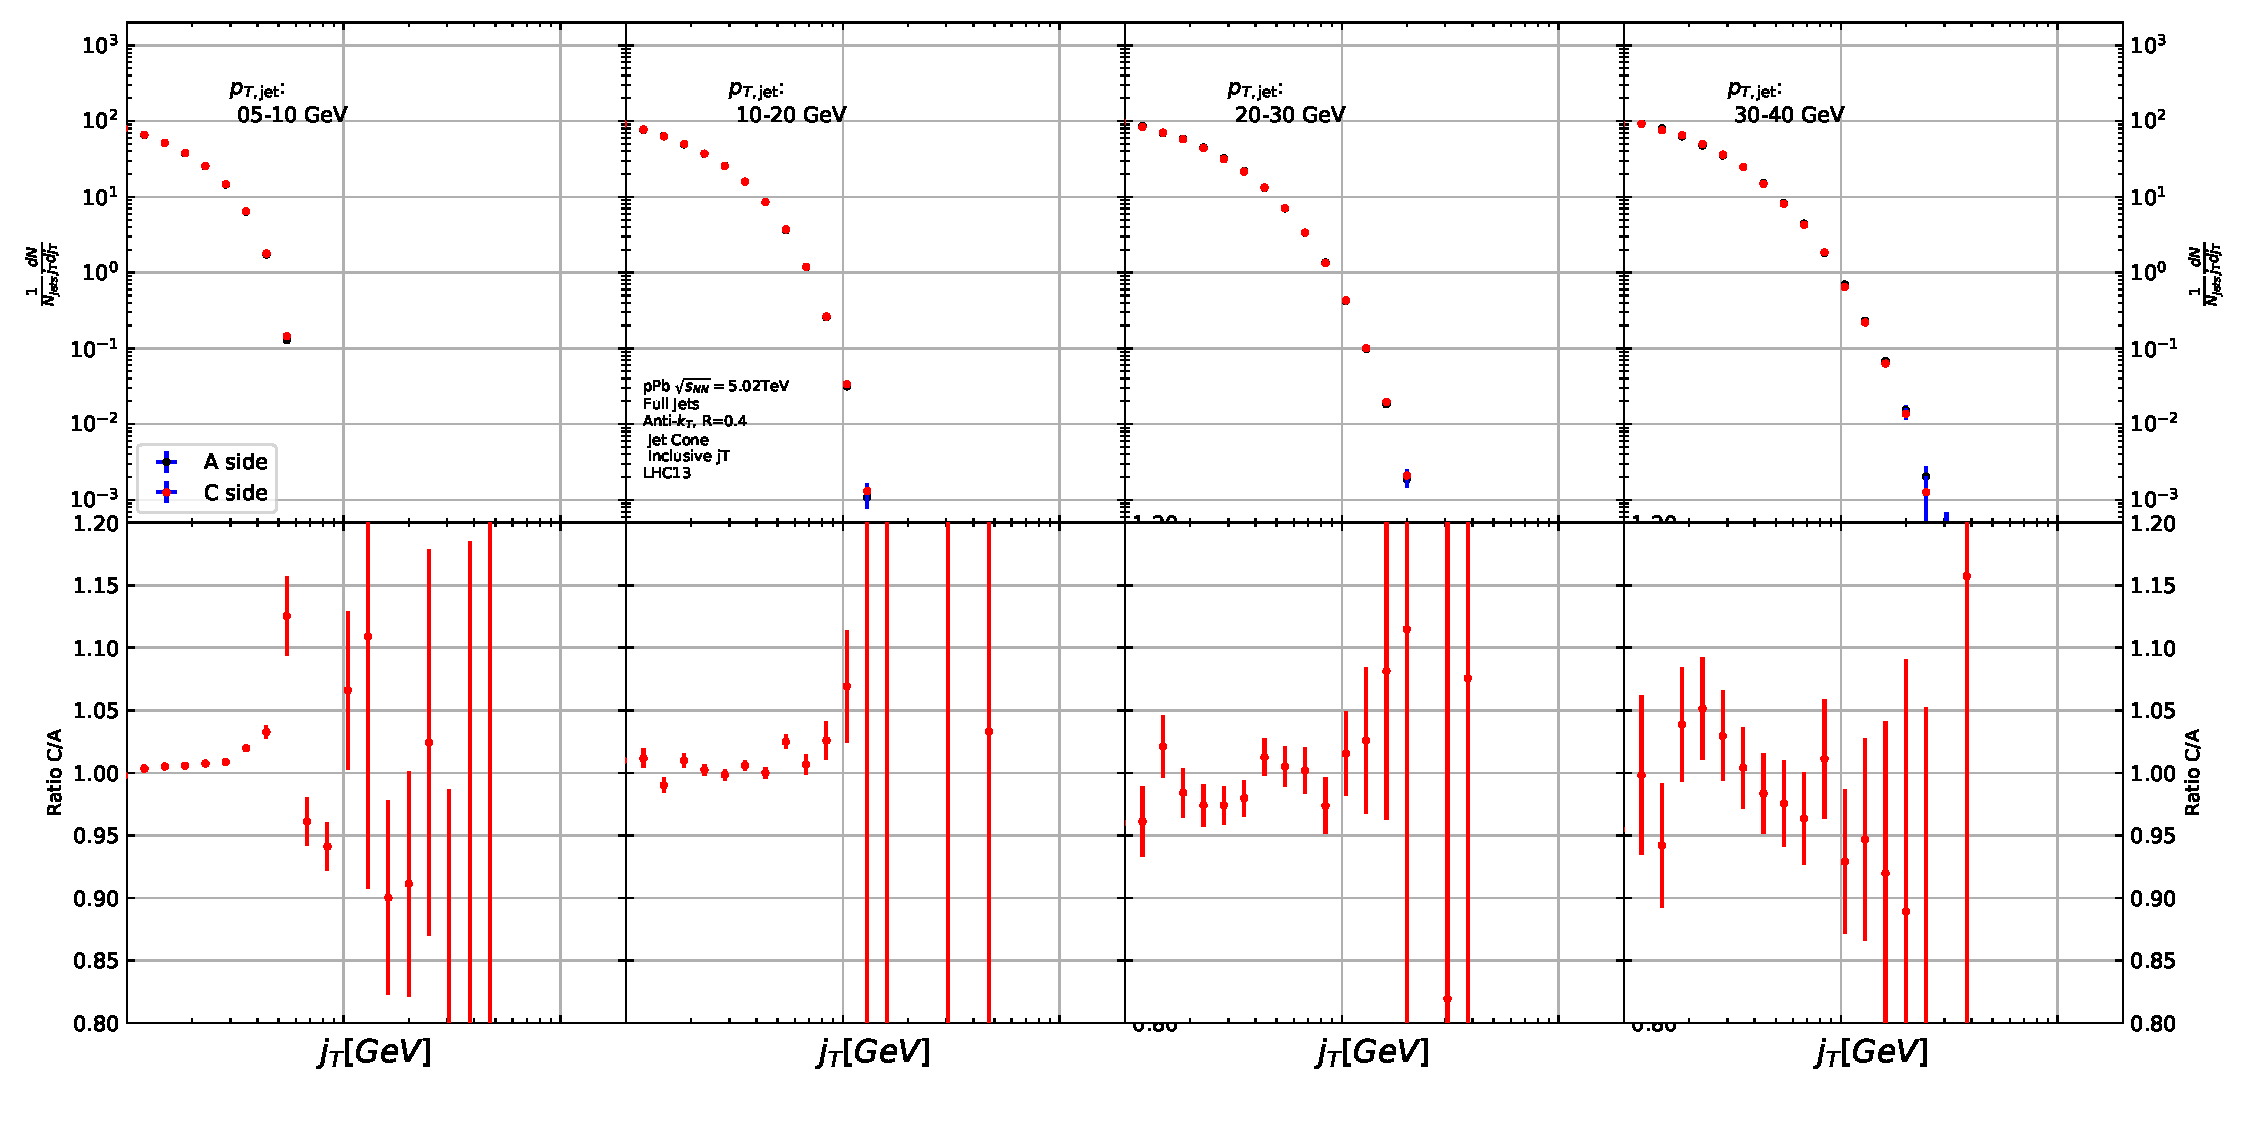
\includegraphics[width=\textwidth]{pics/ACsideComparison/ACsideJetConeJtInclusivePtFrom0To4LHC13.pdf}
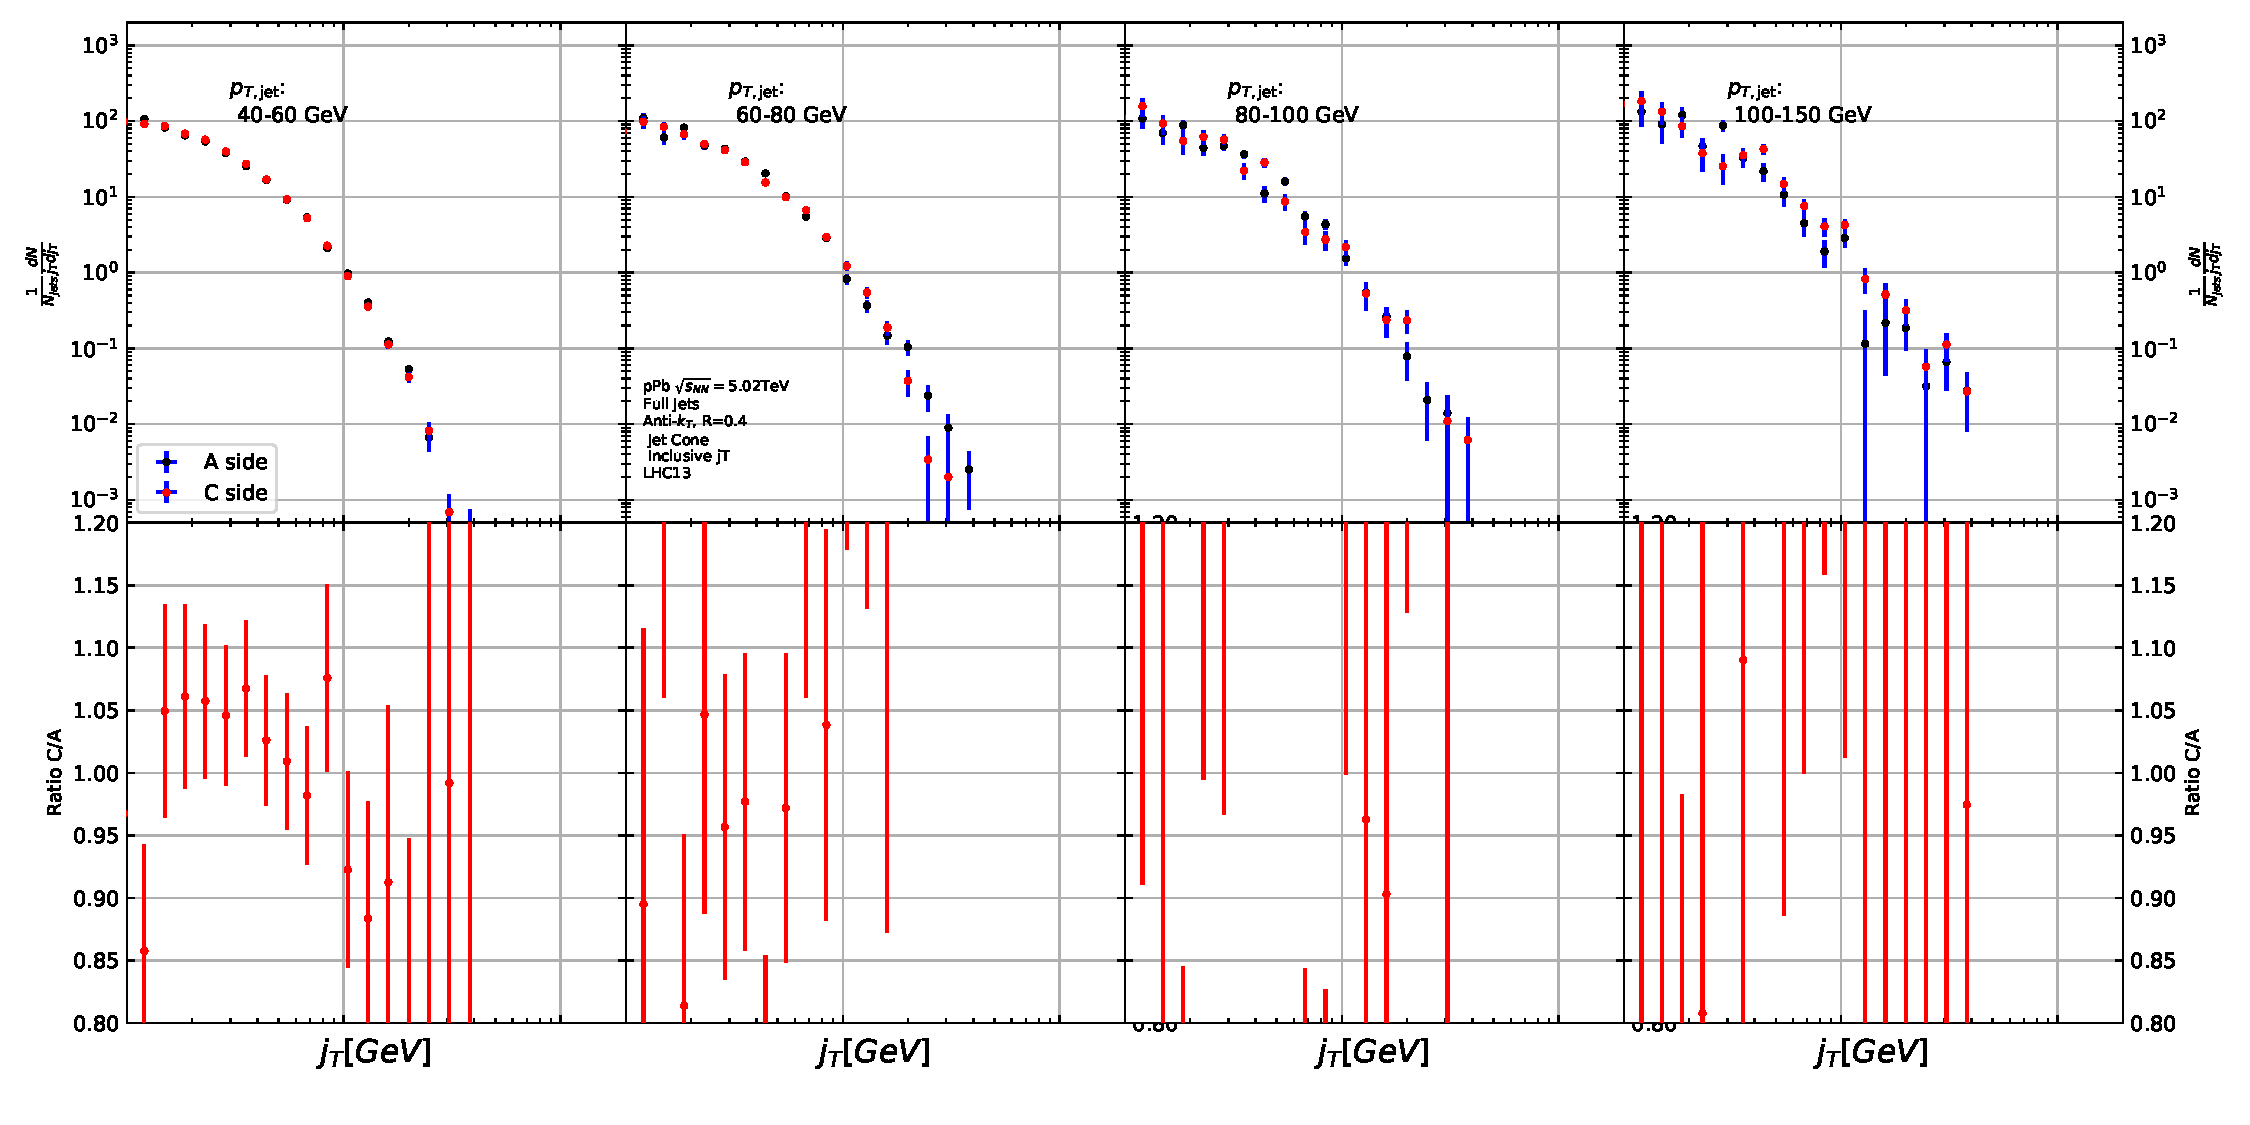
\includegraphics[width=\textwidth]{pics/ACsideComparison/ACsideJetConeJtInclusivePtFrom4To8LHC13.pdf}
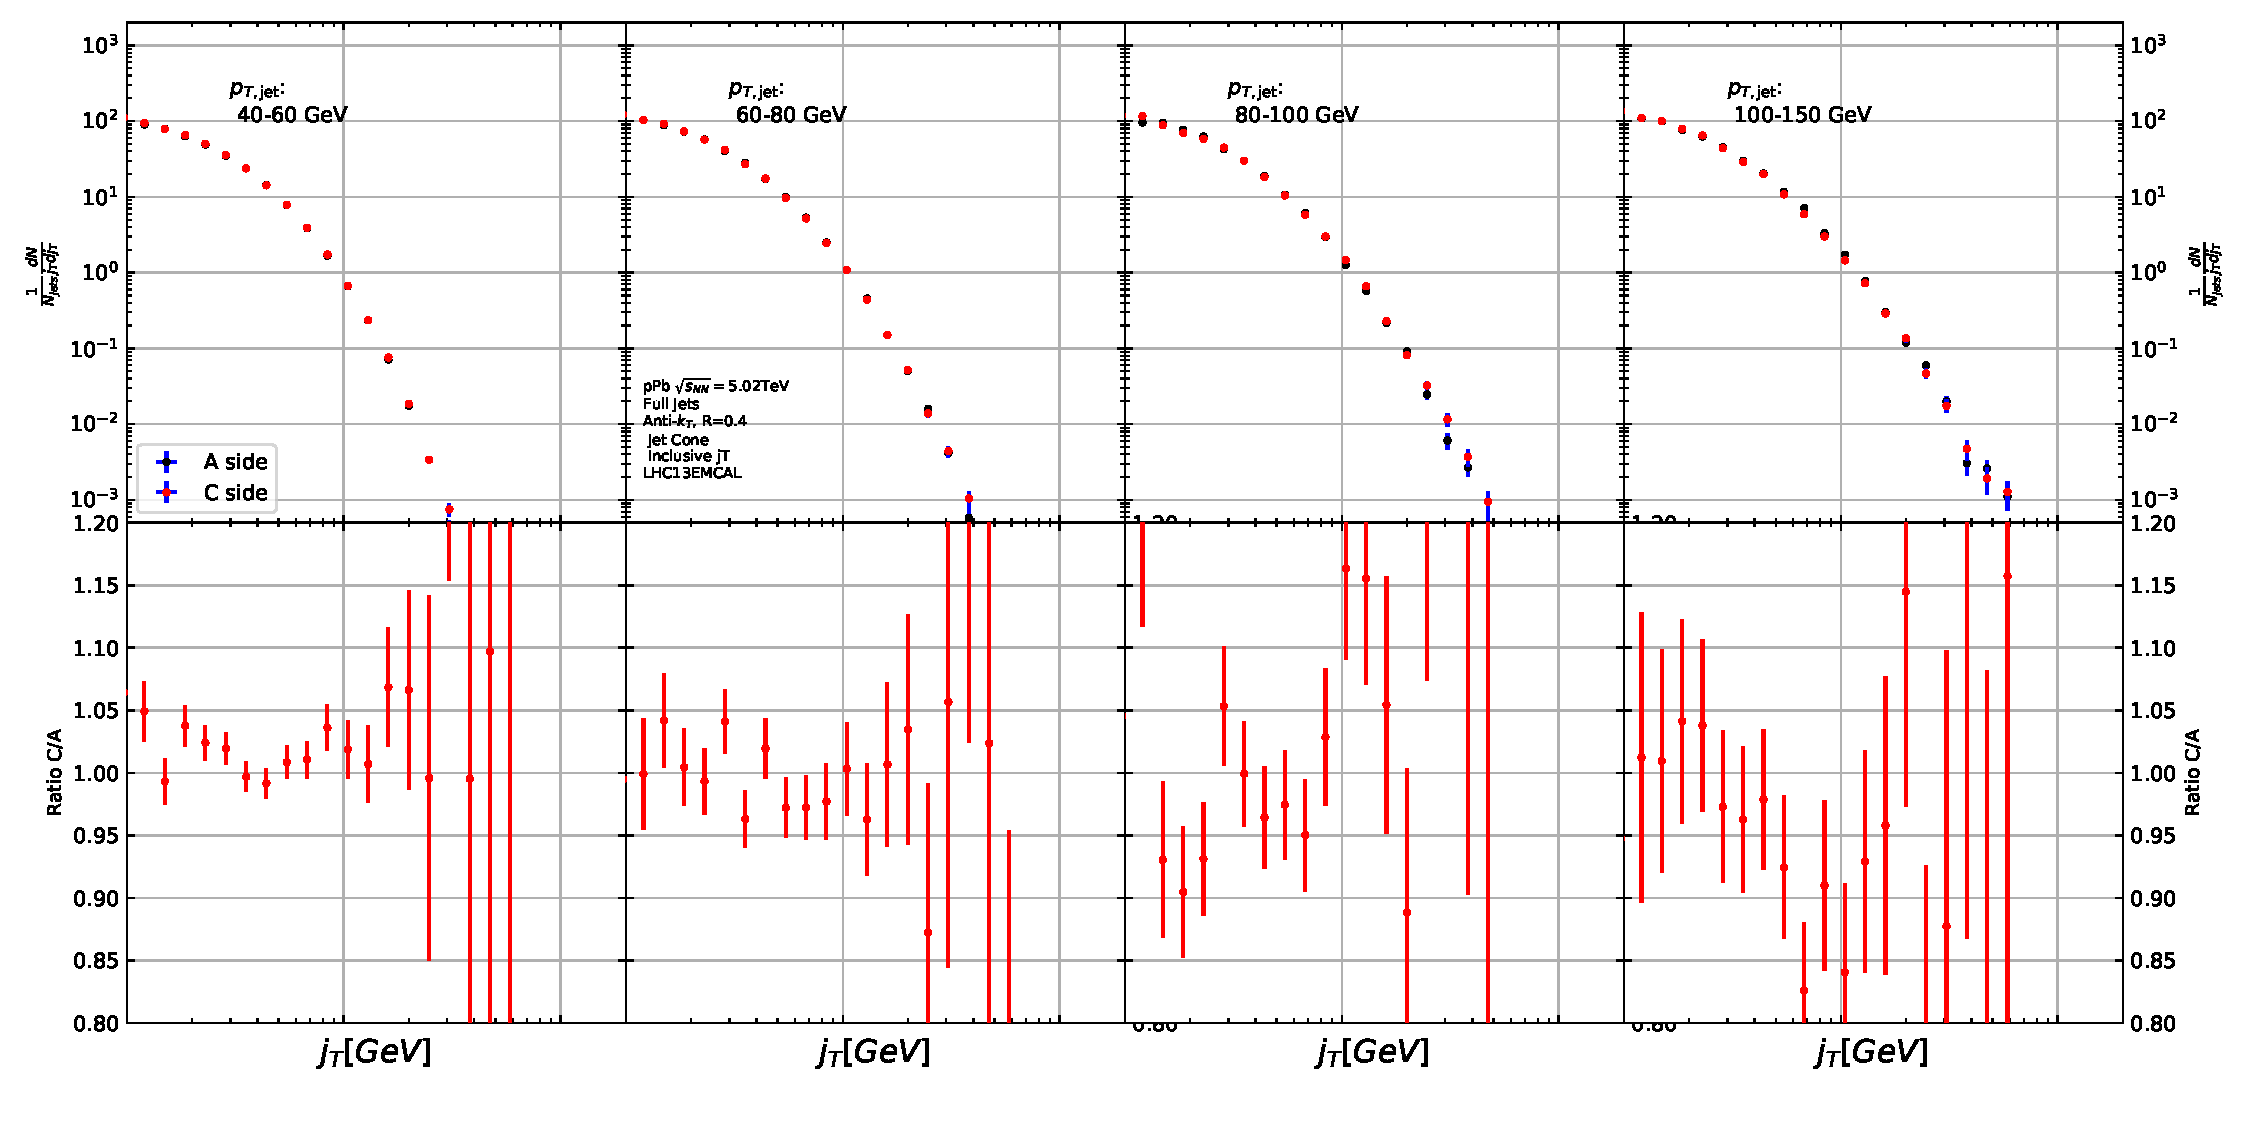
\includegraphics[width=\textwidth]{pics/ACsideComparison/ACsideJetConeJtInclusivePtFrom4To8LHC13EMCAL.pdf}
%Tag 20170810 python2.7 Python/DrawSignal.py legotrain_CF_pPb-1053_20170223-2002_LHC13bcde.root
\end{subfigure}
\caption{Comparison of inclusive $\jt{}$ distributions between A and C side for minimum bias and EMCAL triggered data.}
\label{fig:signalbg}
\end{figure}

\subsection{Subtracted signal}
Results in figure \ref{fig:signal}. Comparison between signals with different backgrounds in figure \ref{fig:signalbg}
\begin{figure}
\centering
\begin{subfigure}{0.95\textwidth}
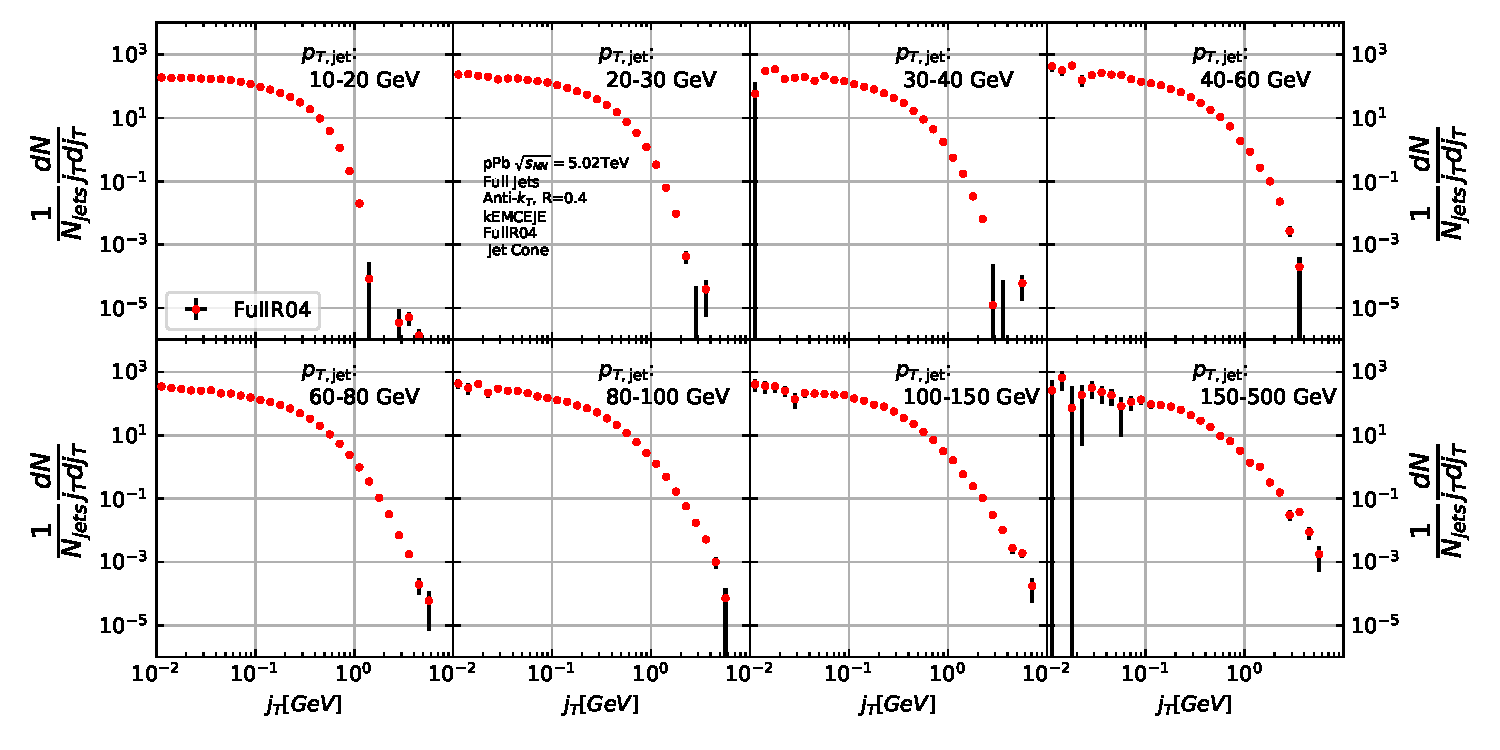
\includegraphics[width=\textwidth]{results/MixedFullJetsR04JetConeJtSignal.pdf}
%Tag 20170810 python2.7 Python/DrawSignal.py legotrain_CF_pPb-1053_20170223-2002_LHC13bcde.root
\end{subfigure}
\caption{$\jt{}$ signal with background subtracted}
\label{fig:signal}
\end{figure}

\begin{figure}
\centering
\begin{subfigure}{0.95\textwidth}
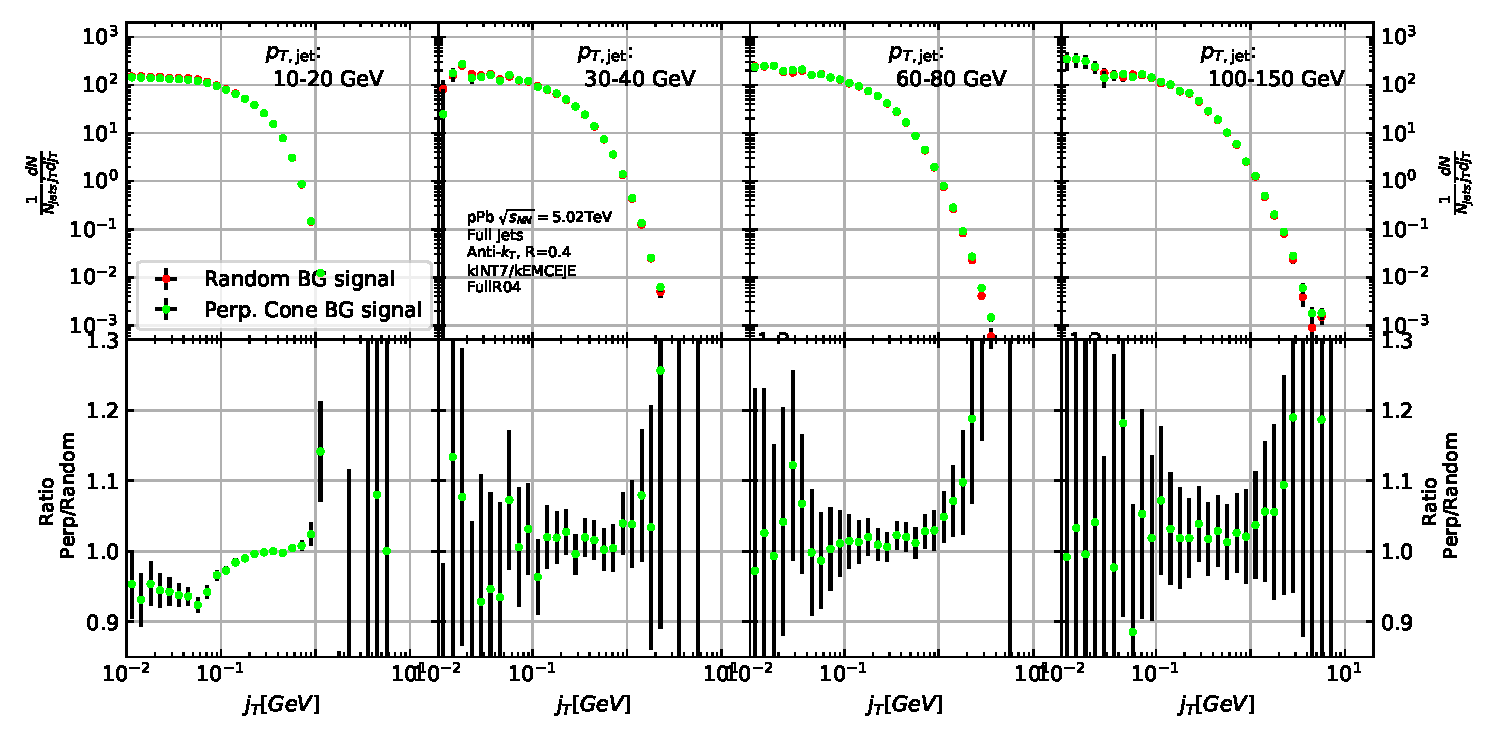
\includegraphics[width=\textwidth]{results/MixedFullJetsR04SignalBackgroundComparison.pdf}
%Tag 20170810 python2.7 Python/DrawSignal.py legotrain_CF_pPb-1053_20170223-2002_LHC13bcde.root
\end{subfigure}
\caption{Comparison of the effect of background method on $\jt{}$ signal.}
\label{fig:signalbg}
\end{figure}



\subsection{Combining systematics}
Resulting systematic erros are shown in table \ref{tab:systematics}. Systematic errors are combined bin-by-bin in quadrature to get the total systematic errors.
\begin{table}[htb]
\centering
\caption{Summary of systematic errors}
\label{tab:systematics}
\begin{tabular}{ l | c | r }
  Systematic & Wide RMS & Narrow RMS \\
    \hline			
  Background & 5 \% & 9 \% \\
  Unfolding & 8 \% & 8 \% \\
  Tracking & \% & \% \\ 
  EMCAL & \% & \% \\
  Total & 9 \% & 12\% \\
  \hline
  \end{tabular}
  \end{table}